\ifx\engineeringnotes\undefined
    \providecommand{\notesroot}{../..}
    \providecommand{\pythonroot}{.}

    \title{Python}
    \author{Donald Cheung\\jianzhang9102@gmail.com}
    \date{\today\footnote{文档编写开始于2018年05月09日}}

    \documentclass[a4paper,10pt]{ctexbook}
\usepackage{xeCJK}
\usepackage{fontspec}
\usepackage{minted}
\usepackage[CJKbookmarks,colorlinks,linkcolor=red]{hyperref}
\usepackage{geometry}
\usepackage{amsmath}
\usepackage[format=hang,font=small,textfont=it]{caption}
\usepackage{float}
\usepackage{subfigure}
\usepackage[nottoc]{tocbibind}
\usepackage{bm}
\usepackage[table, x11names, dvipsnames]{xcolor}
\usepackage{color}
\usepackage{array, booktabs, boldline}
\usepackage{cellspace}
\usepackage{longtable}

\setmainfont{Times New Roman}
\setsansfont{Helvetica}
\setmonofont{Courier New}
\setCJKmainfont[BoldFont={SimHei},ItalicFont={SimHei}]{SimSun}
\setCJKsansfont{SimSun}
\setCJKmonofont{SimSun}

\setcounter{secnumdepth}{4}
\setcounter{tocdepth}{4}

\geometry{left=3.0cm,right=3.0cm,top=2.5cm,bottom=2.5cm}
\bibliographystyle{plain}

%%%%%%%%%%%%%%%%%%%%%%%%%%%%%%%%% minted setting %%%%%%%%%%%%%%%%%%%%%%%%%%%%%%%%%%%
\usemintedstyle{monokai}
\definecolor{bg}{HTML}{282828} % from https://github.com/kevinsawicki/monokai
%\defaultfontfeatures{}
\newfontfamily\noligsmonofamily[NFSSFamily=noligsmonofamily]{Courier}
\setminted{fontfamily=noligsmonofamily}

\renewcommand{\theFancyVerbLine}{%
    \sffamily \textcolor{Dandelion}{\scriptsize \oldstylenums{\arabic{FancyVerbLine}}}}

\newenvironment{jcode}[3]
{%
    \VerbatimEnvironment
    \begin{listing}[h]%
    \caption{#2}%
    \label{#3}%
    \begin{minted}[xleftmargin=18pt,
                   mathescape,
                   linenos,
                   numbersep=5pt,
                   bgcolor=bg,
                   frame=lines,
                   framesep=2mm,
                   fontsize=\footnotesize]{#1}%
}
{%
    \end{minted}
    \vspace{-25pt}%
    \end{listing}%
}
\renewcommand{\listingscaption}{代码}%from minted
\renewcommand{\listoflistingscaption}{代码列表}% from minted


\newenvironment{myquote}{\begin{quote}\kaishu\zihao{-5}}{\end{quote}}
\newcommand\degree{^\circ}
\newtheorem{thm}{定理}


\begin{document}
\maketitle
\tableofcontents
\listoflistings

\else
    \providecommand{\pythonroot}{\engineeringroot/Python}
\fi

\chapter{Python}

\section{Python简介}

\subsection{Python是什么}
Python是著名的``龟叔" Guido van Rossum在1989年圣诞节期间,为了打发无聊的圣诞节而编写的一个编程语言。

现在,全世界差不多有600多种编程语言,但流行的编程语言也就那么20来种。有很多衡量编程语言流行度的方法,比较出名的有TIOBE编程语言排行榜(\ref{fig:TIOBE_INDEX_2017}、\ref{fig:TIOBE_Index_for_January_2017}、\ref{fig:TIOBE_Top10_LANGUAGE_EVOLUTION})、PYPL编程语言人气指数(\ref{fig:PYPL_INDEX_2017}、\ref{fig:PYPL_PopularitY_of_Programming_Language})、RedMonk编程语言排行榜(\ref{fig:REDMONK_RANKING_2017})\footnote{参考链接:\href{https://www.codingame.com/blog/top-programming-languages-to-learn-in-2017/}{TOP PROGRAMMING LANGUAGES TO LEARN IN 2017}}。

\begin{figure}[ht]
  \centering
  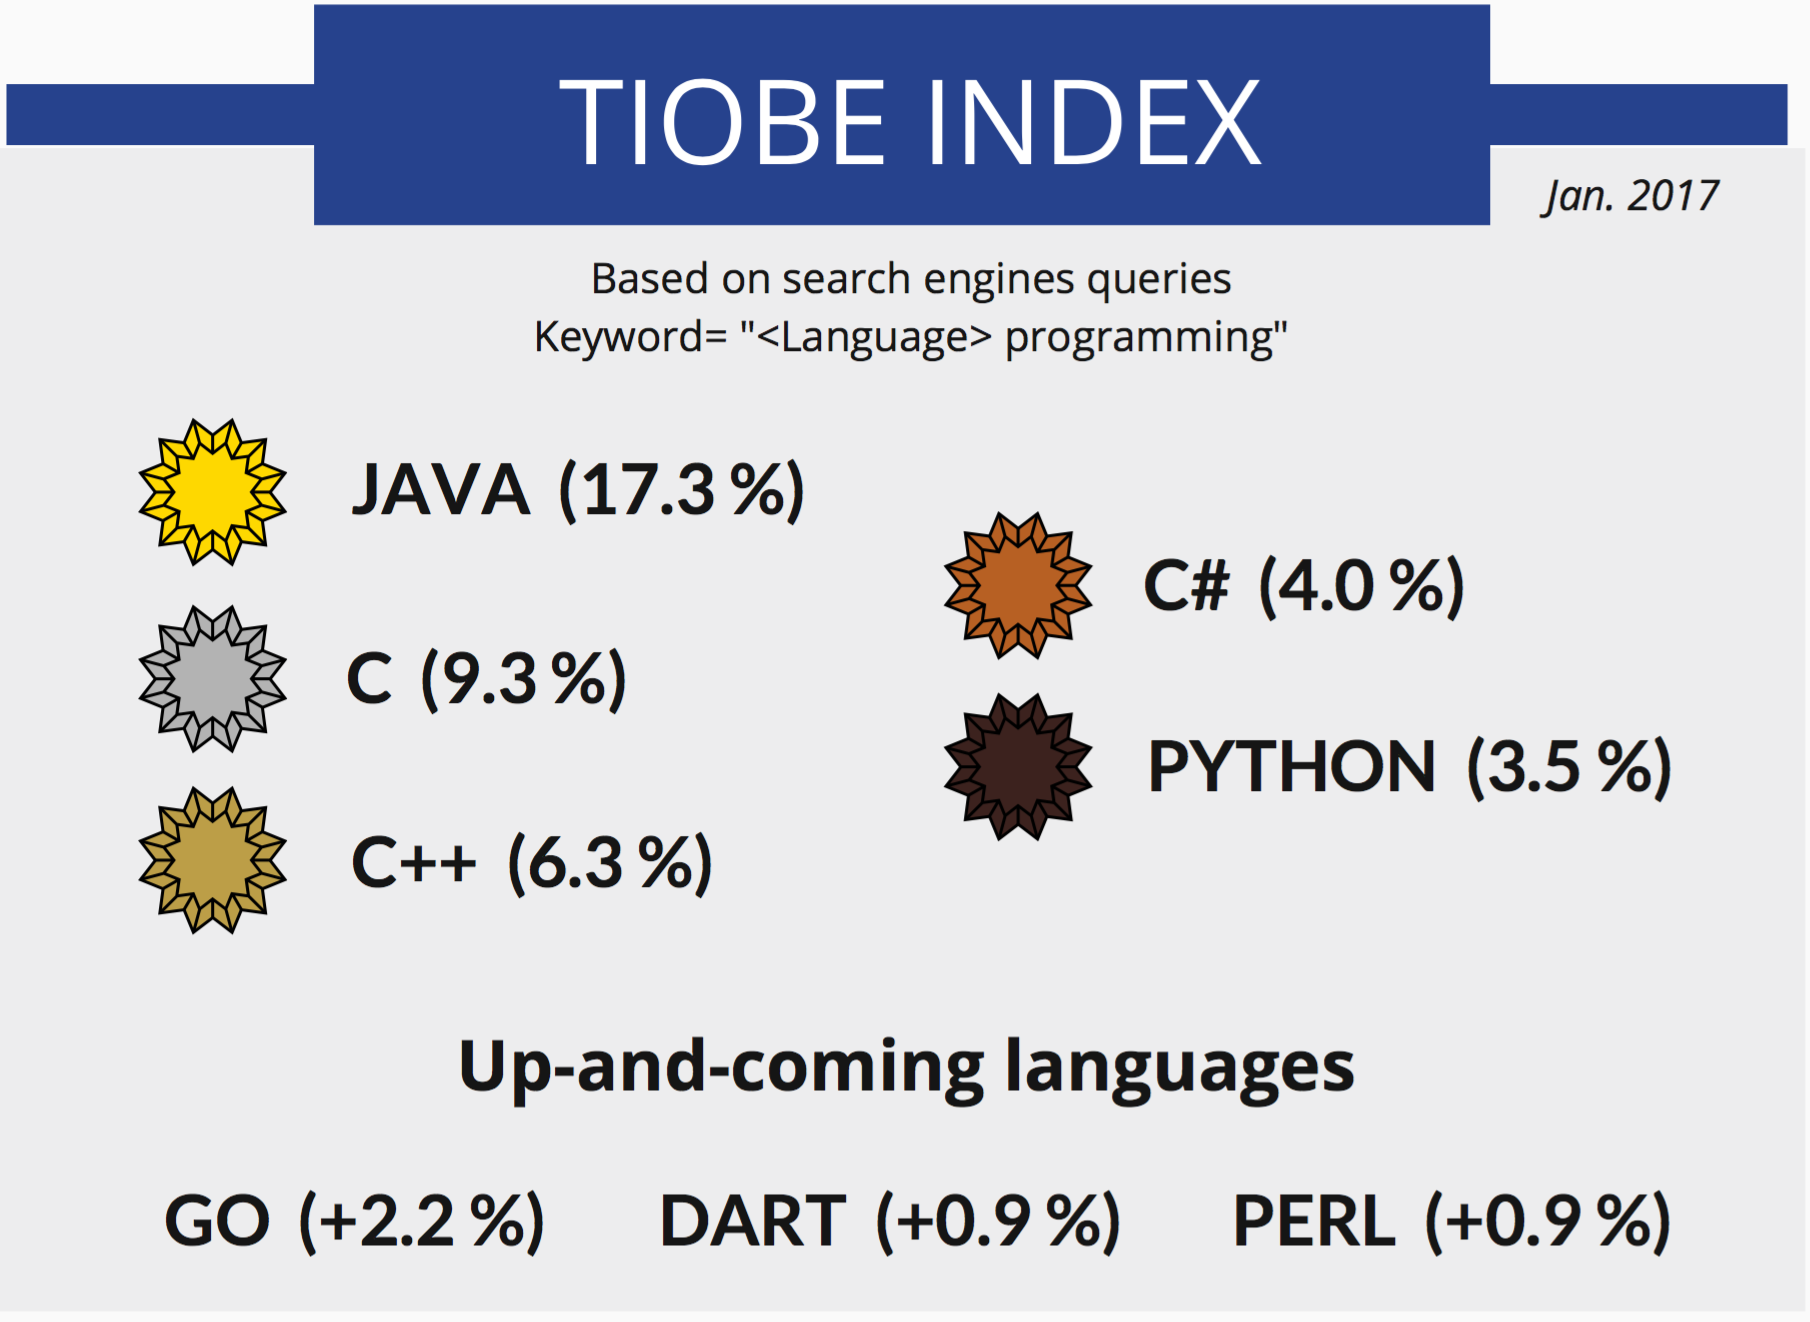
\includegraphics[scale=0.3]{\pythonroot/images/TIOBE_INDEX_2017.png}
  \caption{2017年TIOBE编程语言排行榜}
  \label{fig:TIOBE_INDEX_2017}
\end{figure}

\begin{figure}[ht]
  \centering
  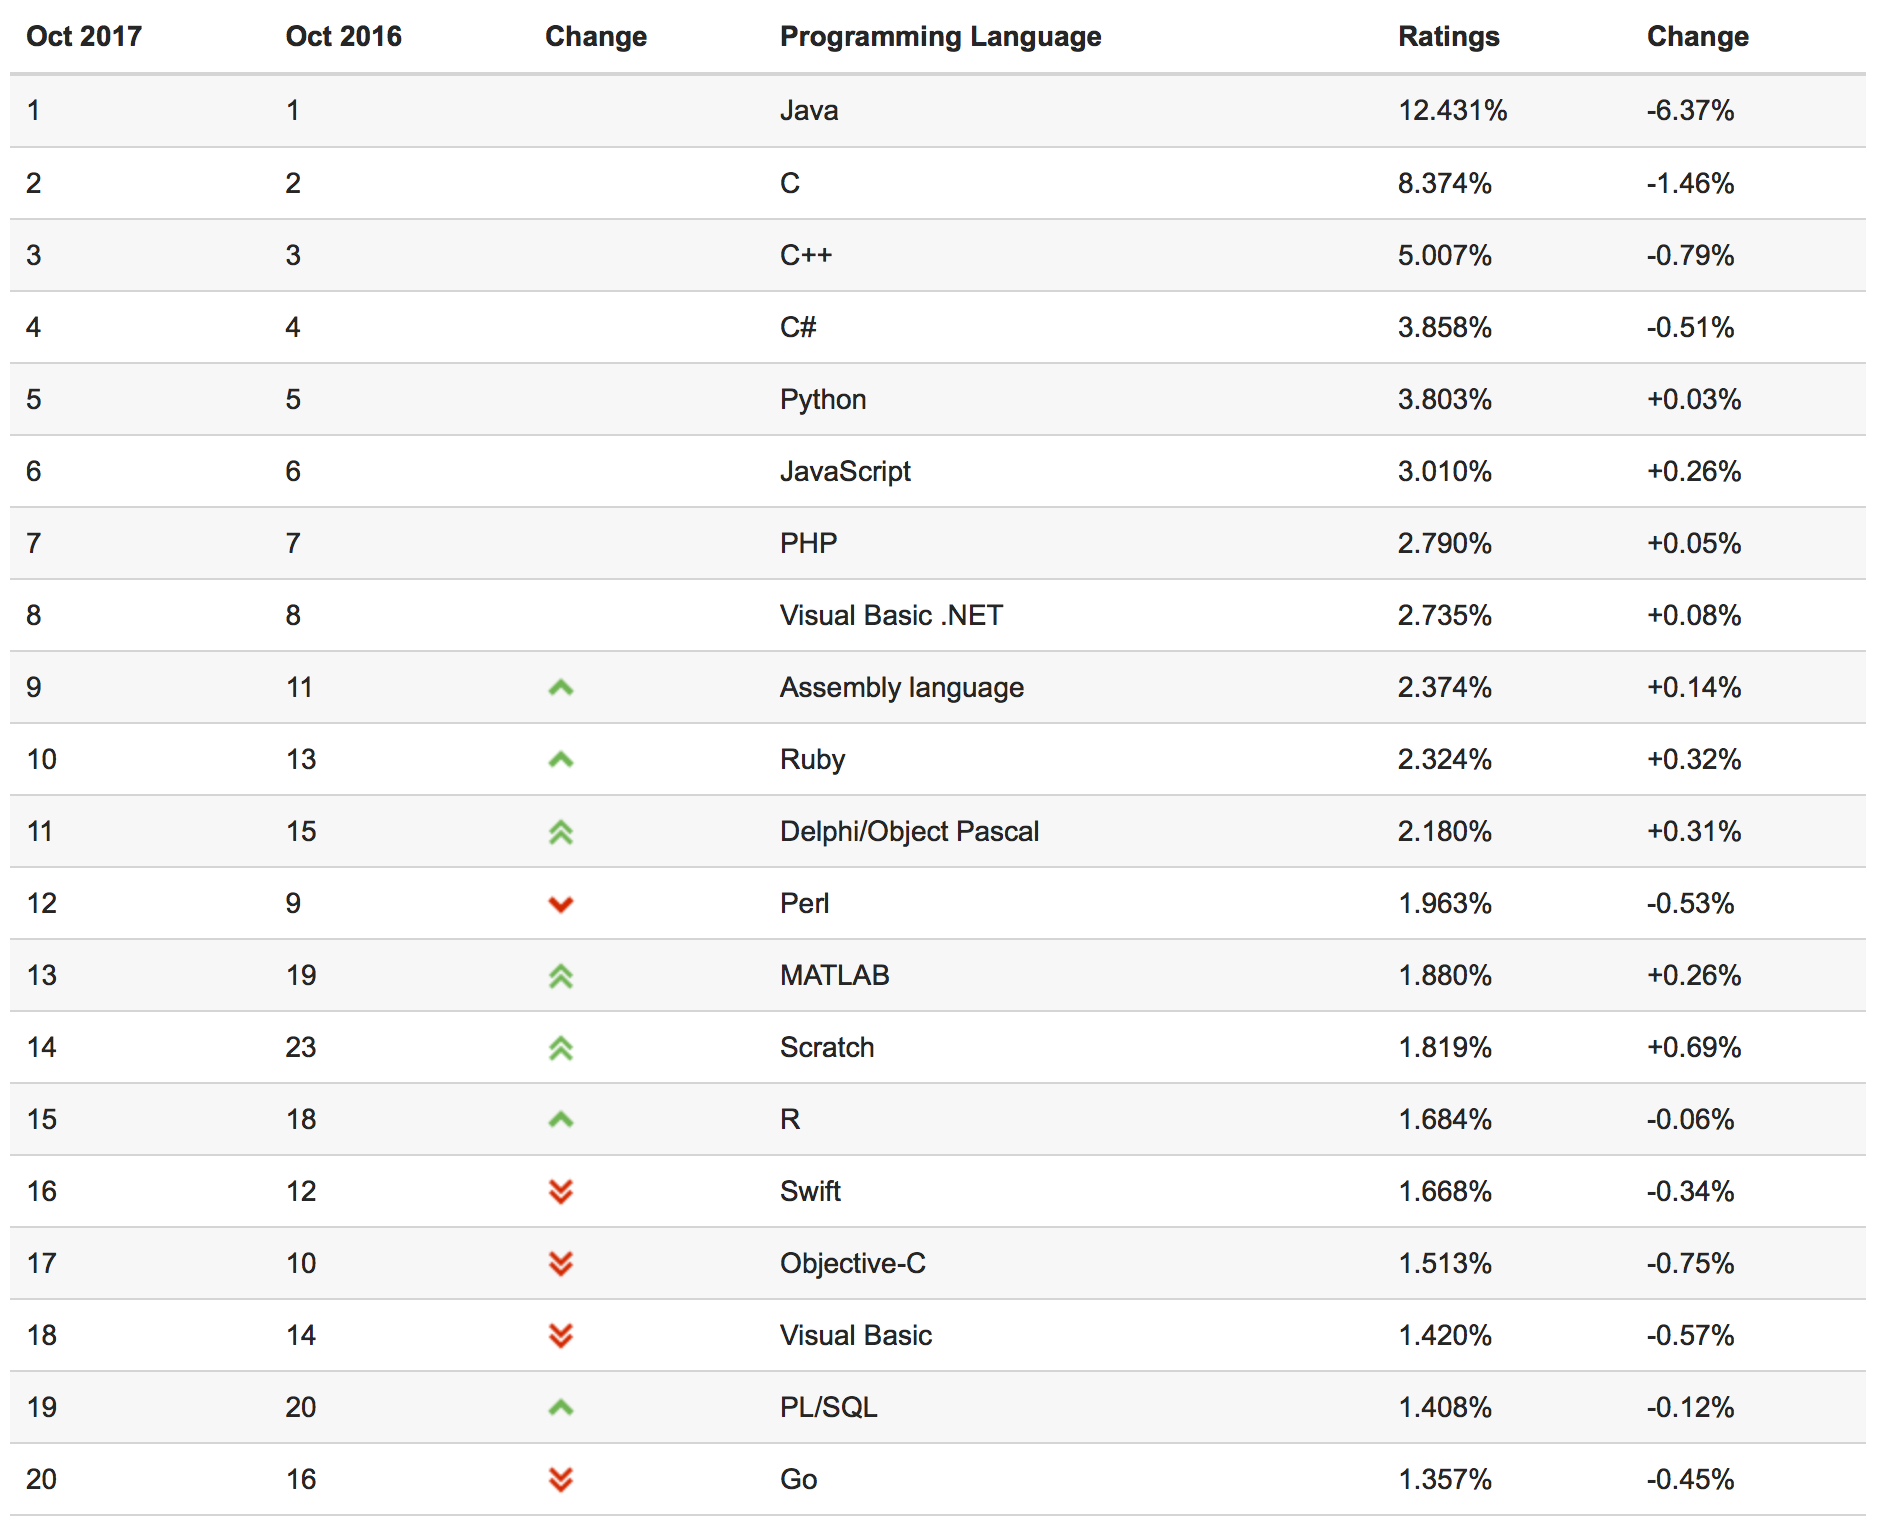
\includegraphics[scale=0.4]{\pythonroot/images/TIOBE_Index_for_January_2017.png}
  \caption{2017年1月TIOBE编程语言排行榜,来源:\href{http://www.tiobe.com/tiobe-index//}{TIOBE Index for January 2017}}
  \label{fig:TIOBE_Index_for_January_2017}
\end{figure}

\begin{figure}[ht]
  \centering
  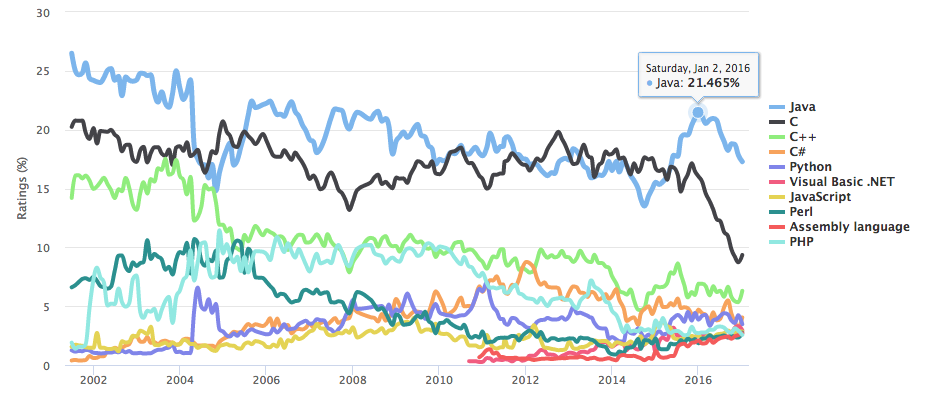
\includegraphics[scale=0.5]{\pythonroot/images/Evolution_of_the_top_10_languages_according_to_Tiobe.png}
  \caption{2017年TIOBE十大编程语言的演变,来源:\href{http://www.tiobe.com/tiobe-index//}{TIOBE Index for January 2017}}
  \label{fig:TIOBE_Top10_LANGUAGE_EVOLUTION}
\end{figure}

\begin{figure}[ht]
  \centering
  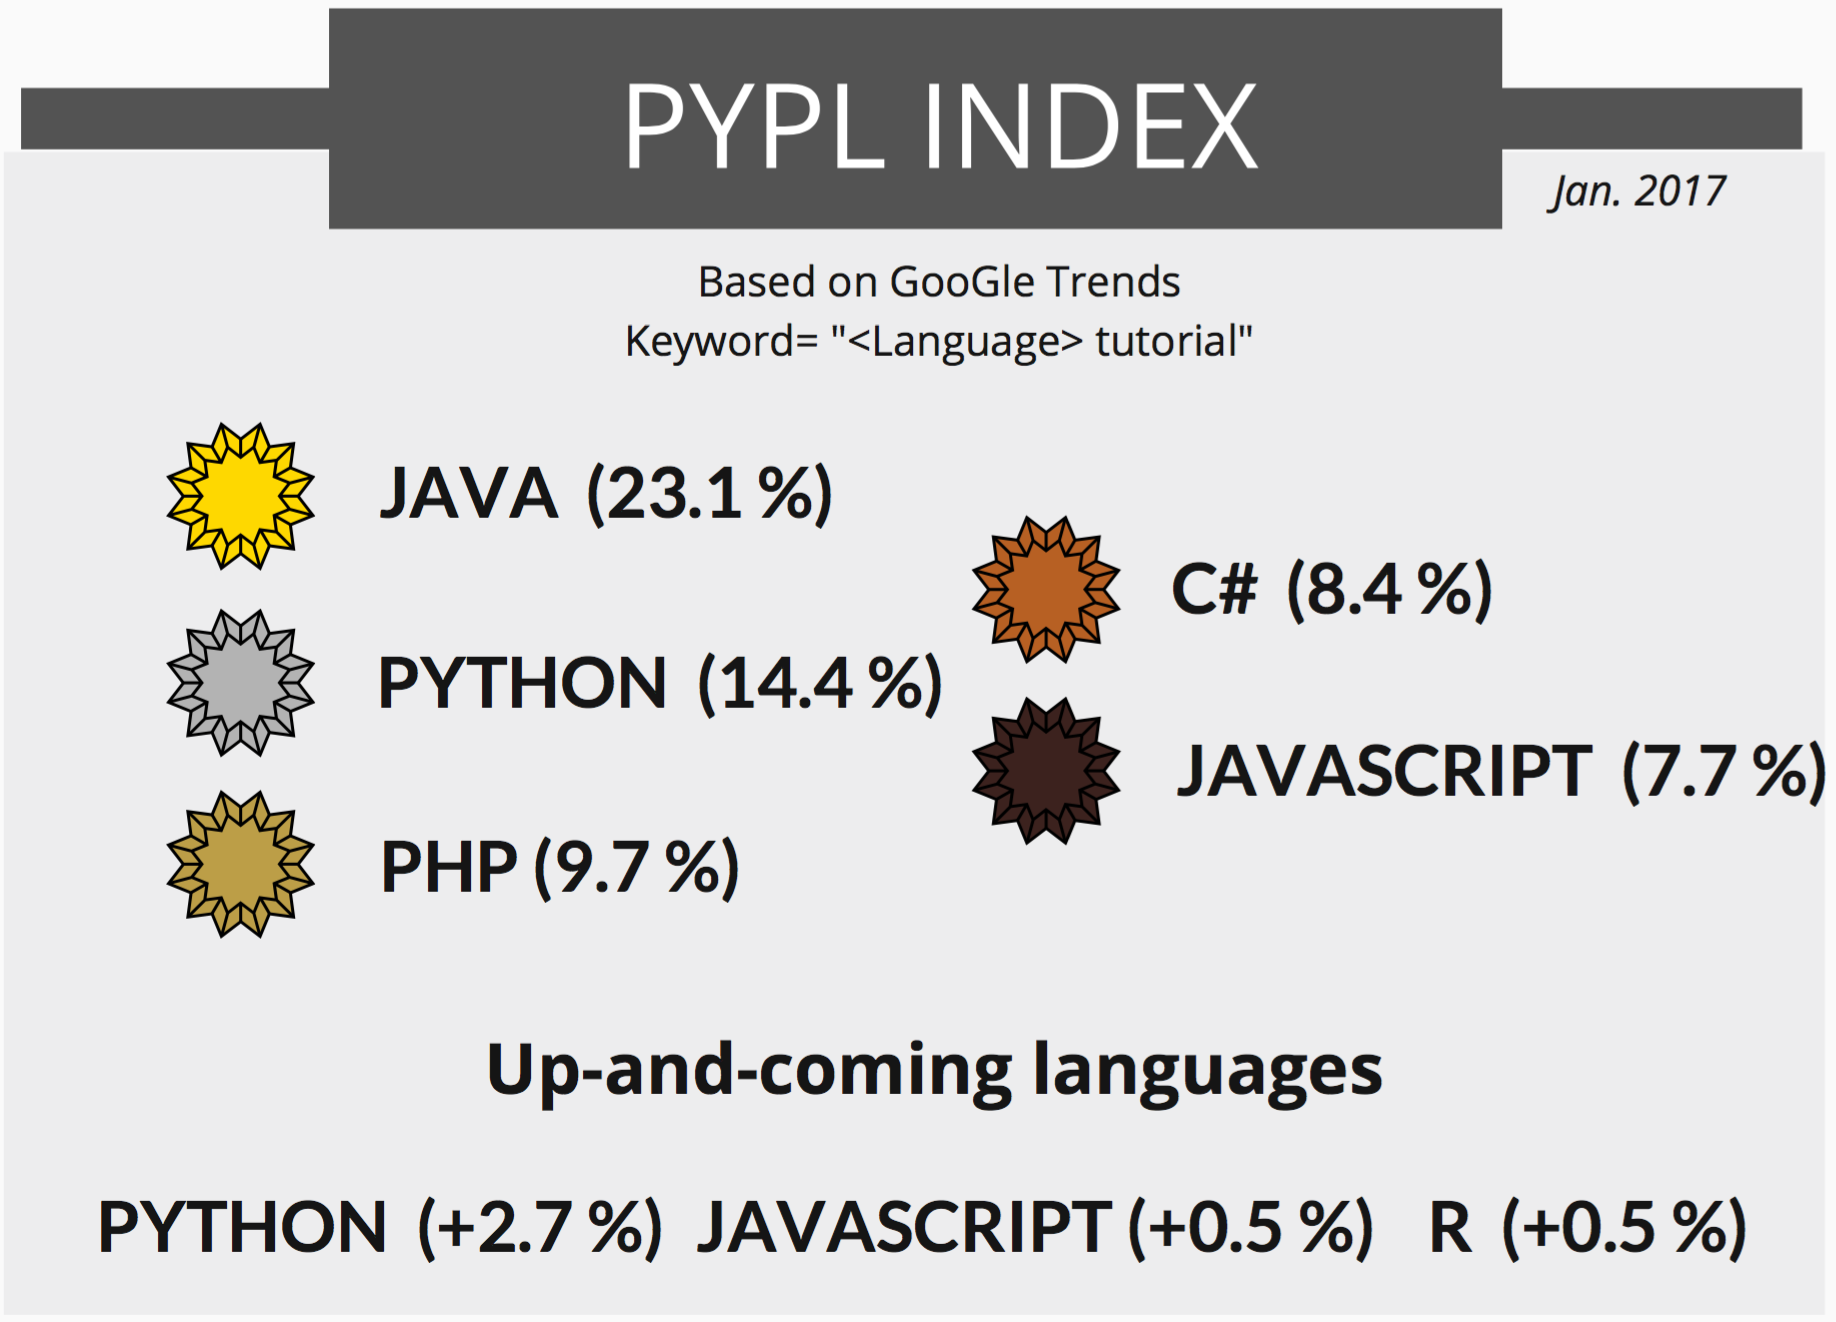
\includegraphics[scale=0.3]{\pythonroot/images/PYPL_INDEX_2017.png}
  \caption{2017年PYPL编程语言人气指数}
  \label{fig:PYPL_INDEX_2017}
\end{figure}

\begin{figure}[ht]
  \centering
  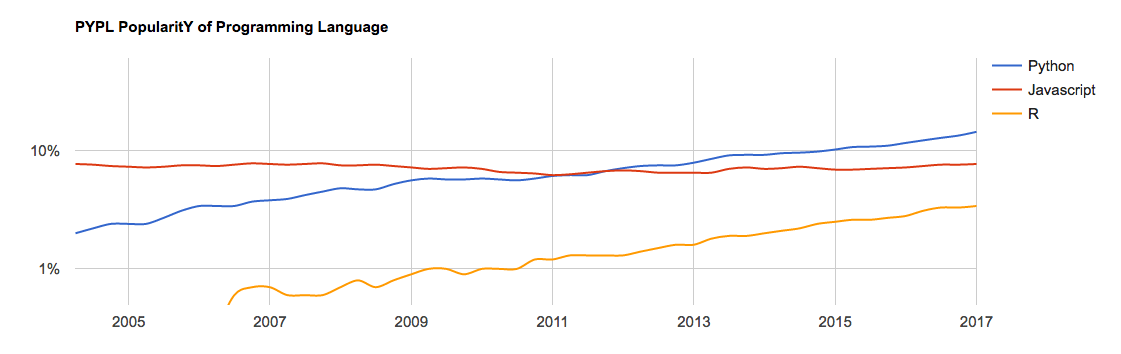
\includegraphics[scale=0.4]{\pythonroot/images/PYPL_PopularitY_of_Programming_Language.png}
  \caption{2017年PYPL编程语言人气指数,来源:\href{http://pypl.github.io/PYPL.html}{PYPL PopularitY of Programming Language Index, January 2017}}
  \label{fig:PYPL_PopularitY_of_Programming_Language}
\end{figure}

\begin{figure}[ht]
  \centering
  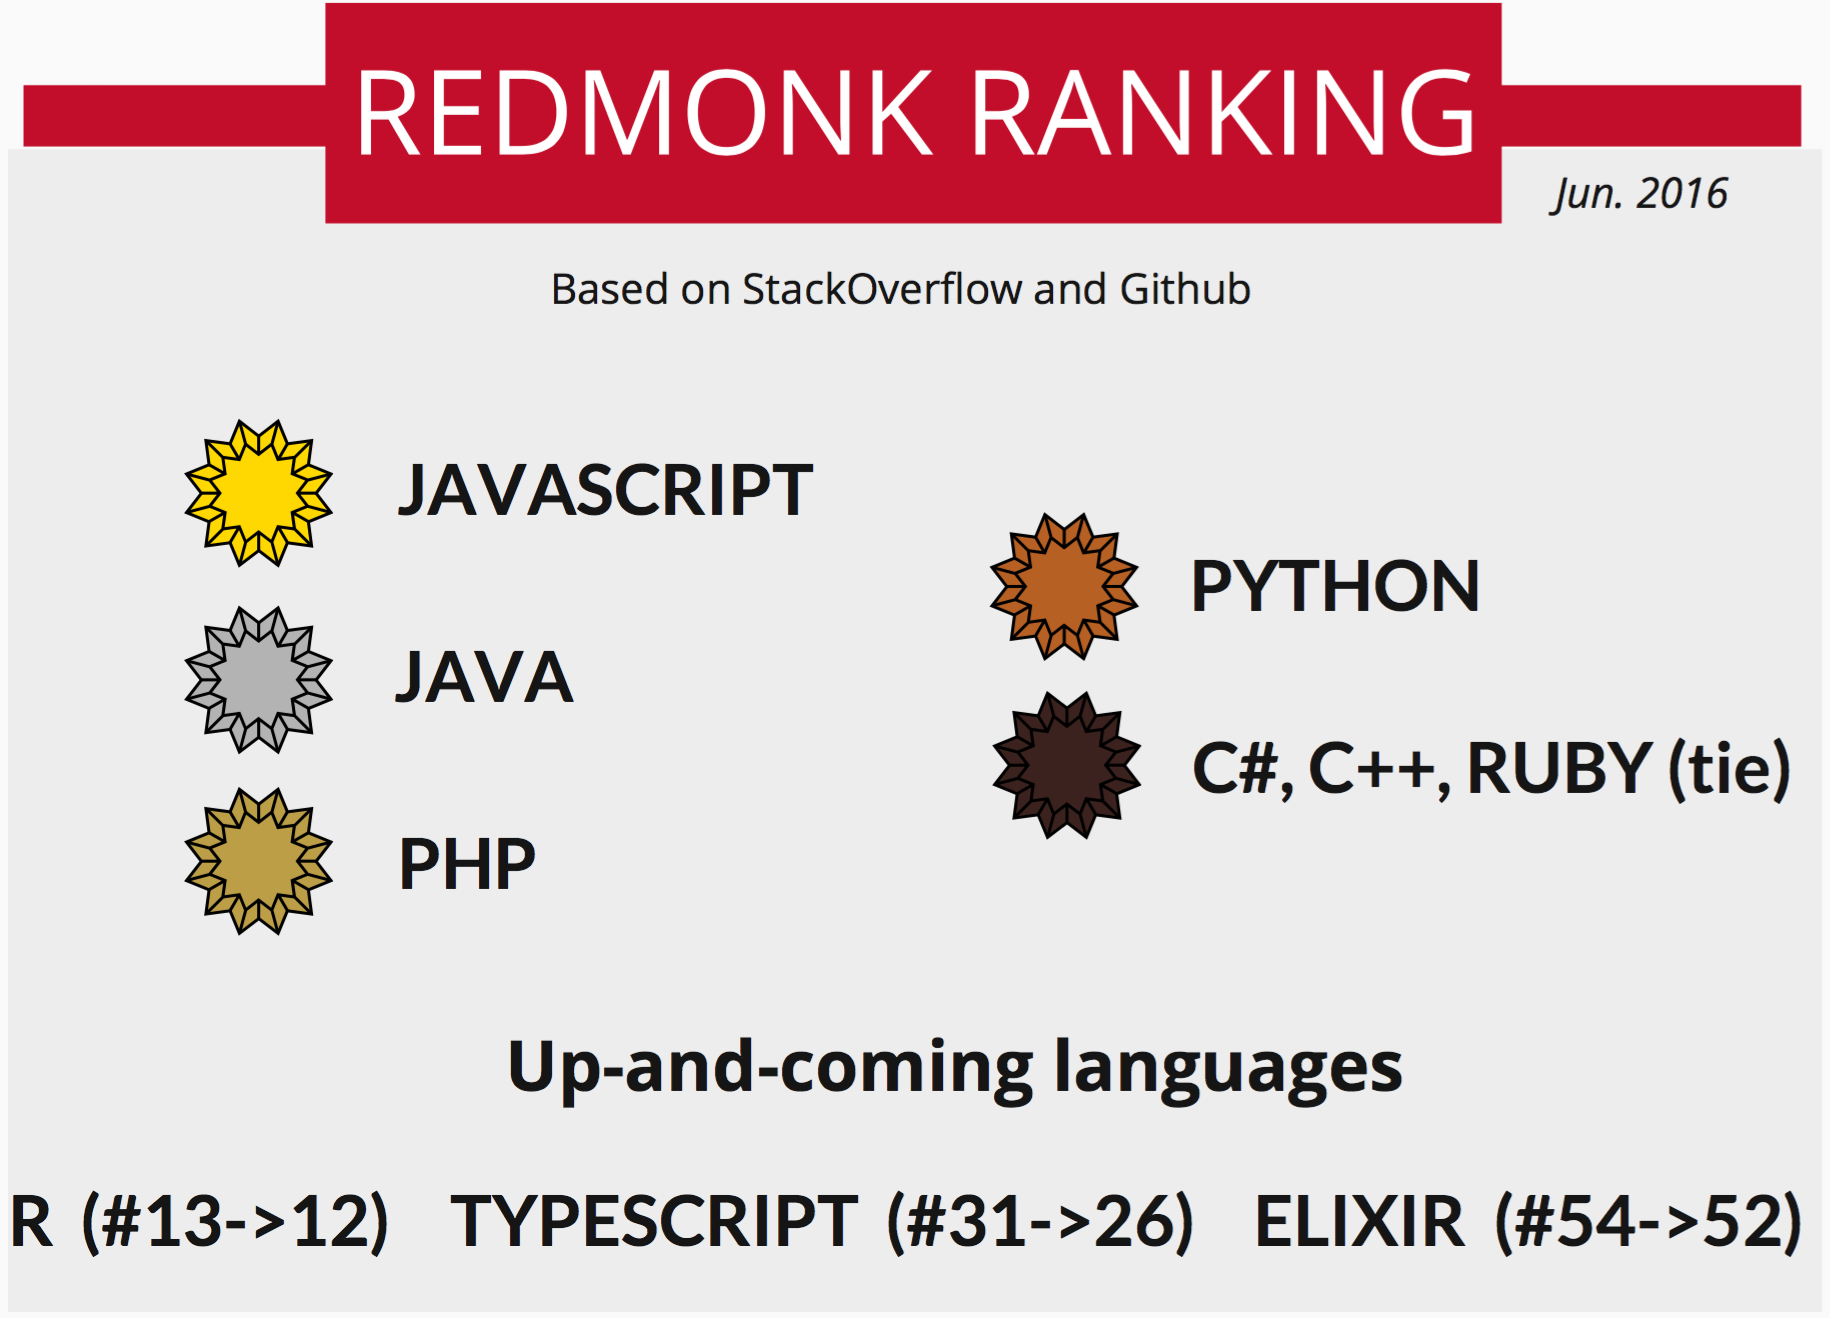
\includegraphics[scale=0.3]{\pythonroot/images/REDMONK_RANKING_2017.png}
  \caption{RedMonk编程语言排行榜}
  \label{fig:REDMONK_RANKING_2017}
\end{figure}

总的来说,这几种编程语言各有千秋。C语言是可以用来编写操作系统的贴近硬件的语言,所以,C语言适合开发那些追求运行速度、充分发挥硬件性能的程序。而Python是用来编写应用程序的高级编程语言。

当你用一种语言开始作真正的软件开发时,你除了编写代码外,还需要很多基本的已经写好的现成的东西,来帮助你加快开发进度。比如说,要编写一个电子邮件客户端,如果先从最底层开始编写网络协议相关的代码,那估计一年半载也开发不出来。高级编程语言通常都会提供一个比较完善的基础代码库,让你能直接调用,比如,针对电子邮件协议的SMTP库,针对桌面环境的GUI库,在这些已有的代码库的基础上开发,一个电子邮件客户端几天就能开发出来。

Python就为我们提供了非常完善的基础代码库,覆盖了网络、文件、GUI、数据库、文本等大量内容,被形象地称作``内置电池(batteries included)"。用Python开发,许多功能不必从零编写,直接使用现成的即可。

除了内置的库外,Python还有大量的第三方库,也就是别人开发的,供你直接使用的东西。当然,如果你开发的代码通过很好的封装,也可以作为第三方库给别人使用。

许多大型网站就是用Python开发的,例如YouTube、Instagram,还有国内的豆瓣。很多大公司,包括Google、Yahoo等,甚至NASA(美国航空航天局)都大量地使用Python。

龟叔给Python的定位是``优雅"、``明确"、``简单",所以Python程序看上去总是简单易懂,初学者学Python,不但入门容易,而且将来深入下去,可以编写那些非常非常复杂的程序。

总的来说,Python的哲学就是简单优雅,尽量写容易看明白的代码,尽量写少的代码。如果一个资深程序员向你炫耀他写的晦涩难懂、动不动就几万行的代码,你可以尽情地嘲笑他。

那Python适合开发哪些类型的应用呢?

首选是网络应用,包括网站、后台服务等等;

其次是许多日常需要的小工具,包括系统管理员需要的脚本任务等等;

另外就是把其他语言开发的程序再包装起来,方便使用。

最后说说Python的缺点。

任何编程语言都有缺点,Python也不例外。优点说过了,那Python有哪些缺点呢?

第一个缺点就是运行速度慢,和C程序相比非常慢,因为Python是解释型语言,你的代码在执行时会一行一行地翻译成CPU能理解的机器码,这个翻译过程非常耗时,所以很慢。而C程序是运行前直接编译成CPU能执行的机器码,所以非常快。

但是大量的应用程序不需要这么快的运行速度,因为用户根本感觉不出来。例如开发一个下载MP3的网络应用程序,C程序的运行时间需要0.001秒,而Python程序的运行时间需要0.1秒,慢了100倍,但由于网络更慢,需要等待1秒,你想,用户能感觉到1.001秒和1.1秒的区别吗?这就好比F1赛车和普通的出租车在北京三环路上行驶的道理一样,虽然F1赛车理论时速高达400公里,但由于三环路堵车的时速只有20公里,因此,作为乘客,你感觉的时速永远是20公里。

不要在意程序运行速度

第二个缺点就是代码不能加密。如果要发布你的Python程序,实际上就是发布源代码,这一点跟C语言不同,C语言不用发布源代码,只需要把编译后的机器码(也就是你在Windows上常见的xxx.exe文件)发布出去。要从机器码反推出C代码是不可能的,所以,凡是编译型的语言,都没有这个问题,而解释型的语言,则必须把源码发布出去。

这个缺点仅限于你要编写的软件需要卖给别人挣钱的时候。好消息是目前的互联网时代,靠卖软件授权的商业模式越来越少了,靠网站和移动应用卖服务的模式越来越多了,后一种模式不需要把源码给别人。

再说了,现在如火如荼的开源运动和互联网自由开放的精神是一致的,互联网上有无数非常优秀的像Linux一样的开源代码,我们千万不要高估自己写的代码真的有非常大的``商业价值"。那些大公司的代码不愿意开放的更重要的原因是代码写得太烂了,一旦开源,就没人敢用他们的产品了。

当然,Python还有其他若干小缺点,请自行忽略,就不一一列举了。

\subsection{安装Python}
因为Python是跨平台的,它可以运行在Windows、Mac和各种Linux/Unix系统上。在Windows上写Python程序,放到Linux上也是能够运行的。

要开始学习Python编程,首先就得把Python安装到你的电脑里。安装后,你会得到Python解释器(就是负责运行Python程序的),一个命令行交互环境,还有一个简单的集成开发环境。

目前,Python有两个版本,一个是2.x版,一个是3.x版,这两个版本是不兼容的,因为现在Python正在朝着3.x版本进化,在进化过程中,大量的针对2.x版本的代码要修改后才能运行,所以,目前有许多第三方库还暂时无法在3.x上使用。

可以通过 python/lib/site-package/myconfig.pth 类似的文件类配置Python的额外库的搜索路径。


\section{Python基础}

\subsection{第一个Python程序}
在交互式环境的提示符>>>下,直接输入代码,按回车,就可以立刻得到代码执行结果。
%\begin{minted}[mathescape, numbersep=5pt, frame=lines, framesep=2mm]{python} 
\begin{jcode}{python}{Python代码示例}{code:yaml-simple-config}
Python 2.7.12 (default, Dec  1 2016, 20:44:50) 
[GCC 4.2.1 Compatible Apple LLVM 8.0.0 (clang-800.0.42.1)] on darwin
Type "help", "copyright", "credits" or "license" for more information.
>>> print 'Hello World'
Hello World
>>> print('Hello World')
Hello World
\end{jcode}

也可以将代码保存在脚本文件中,然后调用python解析器来执行程序。
\begin{minted}[mathescape,
               numbersep=5pt,
               frame=lines,
               framesep=2mm]{python}
$ cat script.py
print 'Hello World'
print('Hello World')

$ python script.py
Hello World
Hello World
\end{minted}

\subsection{Python缩进}
缩进的语句视为代码块,缩进有利有弊。好处是强迫你写出格式化的代码,但没有规定缩进是几个空格还是Tab。按照约定俗成的管理,应该始终坚持使用4个空格的缩进。

缩进的另一个好处是强迫你写出缩进较少的代码,你会倾向于把一段很长的代码拆分成若干函数,从而得到缩进较少的代码。

缩进的坏处就是“复制-粘贴”功能失效了,这是最坑爹的地方。当你重构代码时,粘贴过去的代码必须重新检查缩进是否正确。此外,IDE很难像格式化Java代码那样格式化Python代码。

\subsection{Python标识符}
在Python里,标识符由字母、数字、下划线组成,区分大小写并且不能以数字开头。以下划线开头的标识符是有特殊意义的。以单下划线开头\_foo的代表不能直接访问的类属性,需通过类提供的接口进行访问,不能用from xxx import * 而导入;以双下划线开头的 \_\_foo 代表类的私有成员;以双下划线开头和结尾的 \_\_foo\_\_ 代表 Python 里特殊方法专用的标识,如 \_\_init\_\_() 代表类的构造函数。

Python可以同一行显示多条语句,方法是用分号 ; 分开,如:
\begin{minted}[mathescape,
               numbersep=5pt,
               frame=lines,
               framesep=2mm]{python}
>>> print('hello');print('runoob');
hello
runoob
\end{minted}

\subsection{Python注释}
Python的单行注释使用\#,多行注释采用'''或者""",例如:
\begin{minted}[mathescape,
               linenos,
               numbersep=5pt,
               frame=lines,
               framesep=2mm]{python}
# coding: utf8
# 文件名:test.py

# 第一个注释
print("Hello World")  # 第二个注释
\end{minted}

\begin{minted}[mathescape,
               numbersep=5pt,
               framesep=2mm]{python}
$ python test.py
Hello World
$ 
\end{minted}

\begin{minted}[mathescape,
               %linenos,
               numbersep=5pt,
               frame=lines,
               framesep=2mm]{python}
# coding: utf8
# 文件名:test.py

'''
这是多行注释,使用单引号。
这是多行注释,使用单引号。
这是多行注释,使用单引号。
'''

"""
这是多行注释,使用双引号。
这是多行注释,使用双引号。
这是多行注释,使用双引号。
"""
\end{minted}

\subsection{Python数据类型}

\subsubsection{字符串}

\begin{minted}[mathescape,
               %linenos,
               numbersep=5pt,
               frame=lines,
               framesep=2mm]{python}

>>> s = 'Hello World'
>>> print(s)           # 输出完整字符串
Hello World
>>> print(s[0])        # 输出字符串中的第一个字符
H
>>> print(s[2:5])      # 输出字符串中第三个至第五个之间的字符串
llo
>>> print(s[2:])       # 输出从第三个字符开始的字符串
llo World
>>> print(s * 2)       # 输出字符串两次
Hello WorldHello World
>>> print(s + "TEST")  # 输出连接的字符串
Hello WorldTEST
\end{minted}

\begin{minted}[mathescape,
               %linenos,
               numbersep=5pt,
               frame=lines,
               framesep=2mm]{python}
from __future__ import division
from __future__ import print_function
...
\end{minted}

\subsubsection{列表}

\begin{minted}[mathescape,
               %linenos,
               numbersep=5pt,
               frame=lines,
               framesep=2mm]{python}

>>> lt = ['runoob', 786, 2.23, 'john', 70.2]
>>> tinylist = [123, 'john']
>>> print(lt)               # 输出完整列表
['runoob', 786, 2.23, 'john', 70.2]
>>> print(lt[0])            # 输出列表的第一个元素
runoob
>>> print(lt[1:3])          # 输出第二个至第三个的元素 
[786, 2.23]
>>> print(lt[2:])           # 输出从第三个开始至列表末尾的所有元素
[2.23, 'john', 70.2]
>>> print(tinylist * 2)     # 输出列表两次
[123, 'john', 123, 'john']
>>> print(lt + tinylist)    # 打印组合的列表
['runoob', 786, 2.23, 'john', 70.2, 123, 'john']
\end{minted}

\subsubsection{字典}

\begin{minted}[mathescape, numbersep=5pt, frame=lines, framesep=2mm]{python}
>>> d = {}
>>> d['one'] = "This is one"
>>> d[2] = "This is two"
>> tinydict = {'name': 'john','code':6734, 'dept': 'sales'}
>>> print(d['one'])          # 输出键为'one' 的值
This is one
>>> print(d[2])              # 输出键为 2 的值
This is two
>>> print(tinydict)          # 输出完整的字典
{'dept': 'sales', 'code': 6734, 'name': 'john'}
>>> print(tinydict.keys())   # 输出所有键
['dept', 'code', 'name']
>>> print(tinydict.values()) # 输出所有值
['sales', 6734, 'john']
\end{minted}

\subsubsection{循环控制语句}

\begin{minted}[mathescape, numbersep=5pt, frame=lines, framesep=2mm]{python}
if 判断条件一:
    执行语句一 ...
elif 判断条件二:
    执行语句二 ...
else:
    执行语句三 ...
\end{minted}

\begin{minted}[mathescape, numbersep=5pt, frame=lines, framesep=2mm]{python}
while 判断条件:
    执行语句……
\end{minted}

\begin{minted}[mathescape, numbersep=5pt, frame=lines, framesep=2mm]{python}
for iterating_var in sequence:
    statements(s)
\end{minted}

\subsubsection{函数定义}

你可以定义一个由自己想要功能的函数,以下是简单的规则:
\begin{itemize}
\item 函数代码块以 def 关键词开头,后接函数标识符名称和圆括号()。
\item 任何传入参数和自变量必须放在圆括号中间。圆括号之间可以用于定义参数。
\item 函数的第一行语句可以选择性地使用文档字符串—用于存放函数说明。
\item 函数内容以冒号起始,并且缩进。
\item return [表达式] 结束函数,选择性地返回一个值给调用方。不带表达式的return相当于返回 None。
\end{itemize}

\begin{minted}[mathescape, numbersep=5pt, frame=lines, framesep=2mm]{python}
def functionname(parameters):
    "函数_文档字符串"
    function_suite
    return [expression]
\end{minted}

\subsubsection{特殊函数}

Python内置了一些特殊函数,这些函数很具python特性。可以让代码更加简洁。

\begin{enumerate}
\item filter(function, sequence):
\begin{minted}[mathescape, numbersep=5pt, frame=lines, framesep=2mm]{python}
# Python 2
s = ['a', 'b', 'c', 'd']
def fun1(s):
    return True if s != 'a' else False
ret = filter(fun1, s)
print(ret)
## ['b', 'c', 'd']
\end{minted}

\begin{minted}[mathescape, numbersep=5pt, frame=lines, framesep=2mm]{python}
# Python 3
s = ['a', 'b', 'c', 'd']
def fun1(s):
    return True if s != 'a' else False
ret = filter(fun1, s)
print(ret)
# <filter object at 0x106490940>
print(list(ret))
## ['b', 'c', 'd']
\end{minted}

对sequence中的item依次执行function(item),将执行结果为True的item组成一个List/String/Tuple(取决于sequence的类型)返回。
可以看作是过滤函数。

\item map(function, sequence) 
\begin{minted}[mathescape, numbersep=5pt, frame=lines, framesep=2mm]{python}
# Python 2
s = ['a', 'b', 'c', 'd'] 
def fun2(s):
    return s + ".txt"
ret = map(fun2, s)
print(ret)
# ['a.txt', 'b.txt', 'c.txt', 'd.txt']
\end{minted}

\begin{minted}[mathescape, numbersep=5pt, frame=lines, framesep=2mm]{python}
# Python 3
s = ['a', 'b', 'c', 'd'] 
def fun2(s):
    return s + ".txt"
ret = map(fun2, s)
print(ret)
# <map object at 0x10449ea58>
print(list(ret))
# ['a.txt', 'b.txt', 'c.txt', 'd.txt']
\end{minted}

对sequence中的item依次执行function(item),见执行结果组成一个List返回:

map也支持多个sequence,这就要求function也支持相应数量的参数输入:
\begin{minted}[mathescape, numbersep=5pt, frame=lines, framesep=2mm]{python}
def add(x, y):
    return x + y 

print map(add, range(10), range(10)) 
##[0, 2, 4, 6, 8, 10, 12, 14, 16, 18]
\end{minted}

\item reduce(function, sequence, starting\_value)
\begin{minted}[mathescape, numbersep=5pt, frame=lines, framesep=2mm]{python}
from functools import reduce # for python 3
def add1(x,y):
    return x + y
print(reduce(add1, range(1, 100)))
print(reduce(add1, range(1, 100), 20))
# 4950 (注:1+2+...+99)
# 4970 (注:1+2+...+99+20)
\end{minted}

对sequence中的item顺序迭代调用function,如果有starting\_value,还可以作为初始值调用。
\item lambda:
\begin{minted}[mathescape, numbersep=5pt, frame=lines, framesep=2mm]{python}
g = lambda s: s + ".fsh"
print(g("haha"))
print((lambda x: x * 2)(3))

## haha.fsh
## 6
\end{minted}

这是Python支持一种有趣的语法,它允许你快速定义单行的最小函数,类似与C语言中的宏,这些叫做lambda的函数.
\end{enumerate}

\subsection{使用list和tuple}

使用list和tuple

Reads: 450657
list

Python内置的一种数据类型是列表:list。list是一种有序的集合,可以随时添加和删除其中的元素。

比如,列出班里所有同学的名字,就可以用一个list表示:

%>>> classmates = ['Michael', 'Bob', 'Tracy']
>>> classmates
%['Michael', 'Bob', 'Tracy']
变量classmates就是一个list。用len()函数可以获得list元素的个数:

>>> len(classmates)
3
用索引来访问list中每一个位置的元素,记得索引是从0开始的:

%>>> classmates[0]
'Michael'
%>>> classmates[1]
'Bob'
%>>> classmates[2]
'Tracy'
%>>> classmates[3]
Traceback (most recent call last):
  File "<stdin>", line 1, in <module>
IndexError: list index out of range
当索引超出了范围时,Python会报一个IndexError错误,所以,要确保索引不要越界,记得最后一个元素的索引是len(classmates) - 1。

如果要取最后一个元素,除了计算索引位置外,还可以用-1做索引,直接获取最后一个元素:

>>> classmates[-1]
'Tracy'
以此类推,可以获取倒数第2个、倒数第3个:

>>> classmates[-2]
'Bob'
>>> classmates[-3]
'Michael'
>>> classmates[-4]
Traceback (most recent call last):
  File "<stdin>", line 1, in <module>
IndexError: list index out of range
当然,倒数第4个就越界了。

list是一个可变的有序表,所以,可以往list中追加元素到末尾:

>>> classmates.append('Adam')
>>> classmates
['Michael', 'Bob', 'Tracy', 'Adam']
也可以把元素插入到指定的位置,比如索引号为1的位置:

>>> classmates.insert(1, 'Jack')
>>> classmates
['Michael', 'Jack', 'Bob', 'Tracy', 'Adam']
要删除list末尾的元素,用pop()方法:

>>> classmates.pop()
'Adam'
>>> classmates
['Michael', 'Jack', 'Bob', 'Tracy']
要删除指定位置的元素,用pop(i)方法,其中i是索引位置:

>>> classmates.pop(1)
'Jack'
>>> classmates
['Michael', 'Bob', 'Tracy']
要把某个元素替换成别的元素,可以直接赋值给对应的索引位置:

>>> classmates[1] = 'Sarah'
>>> classmates
['Michael', 'Sarah', 'Tracy']
list里面的元素的数据类型也可以不同,比如:

>>> L = ['Apple', 123, True]
list元素也可以是另一个list,比如:

>>> s = ['python', 'java', ['asp', 'php'], 'scheme']
>>> len(s)
4
要注意s只有4个元素,其中s[2]又是一个list,如果拆开写就更容易理解了:

>>> p = ['asp', 'php']
>>> s = ['python', 'java', p, 'scheme']
要拿到'php'可以写p[1]或者s[2][1],因此s可以看成是一个二维数组,类似的还有三维、四维……数组,不过很少用到。

如果一个list中一个元素也没有,就是一个空的list,它的长度为0:

>>> L = []
>>> len(L)
0
tuple

另一种有序列表叫元组:tuple。tuple和list非常类似,但是tuple一旦初始化就不能修改,比如同样是列出同学的名字:

>>> classmates = ('Michael', 'Bob', 'Tracy')
现在,classmates这个tuple不能变了,它也没有append(),insert()这样的方法。其他获取元素的方法和list是一样的,你可以正常地使用classmates[0],classmates[-1],但不能赋值成另外的元素。

不可变的tuple有什么意义?因为tuple不可变,所以代码更安全。如果可能,能用tuple代替list就尽量用tuple。

tuple的陷阱:当你定义一个tuple时,在定义的时候,tuple的元素就必须被确定下来,比如:

>>> t = (1, 2)
>>> t
(1, 2)
如果要定义一个空的tuple,可以写成():

>>> t = ()
>>> t
()
但是,要定义一个只有1个元素的tuple,如果你这么定义:

>>> t = (1)
>>> t
1
定义的不是tuple,是1这个数!这是因为括号()既可以表示tuple,又可以表示数学公式中的小括号,这就产生了歧义,因此,Python规定,这种情况下,按小括号进行计算,计算结果自然是1。

所以,只有1个元素的tuple定义时必须加一个逗号,,来消除歧义:

>>> t = (1,)
>>> t
(1,)
Python在显示只有1个元素的tuple时,也会加一个逗号,,以免你误解成数学计算意义上的括号。

最后来看一个“可变的”tuple:

>>> t = ('a', 'b', ['A', 'B'])
>>> t[2][0] = 'X'
>>> t[2][1] = 'Y'
>>> t
('a', 'b', ['X', 'Y'])
这个tuple定义的时候有3个元素,分别是'a','b'和一个list。不是说tuple一旦定义后就不可变了吗?怎么后来又变了?

别急,我们先看看定义的时候tuple包含的3个元素:

tuple-0

当我们把list的元素'A'和'B'修改为'X'和'Y'后,tuple变为:

tuple-1

表面上看,tuple的元素确实变了,但其实变的不是tuple的元素,而是list的元素。tuple一开始指向的list并没有改成别的list,所以,tuple所谓的“不变”是说,tuple的每个元素,指向永远不变。即指向'a',就不能改成指向'b',指向一个list,就不能改成指向其他对象,但指向的这个list本身是可变的!

理解了“指向不变”后,要创建一个内容也不变的tuple怎么做?那就必须保证tuple的每一个元素本身也不能变。

小结

list和tuple是Python内置的有序集合,一个可变,一个不可变。根据需要来选择使用它们。

\subsection{条件判断和循环}
条件判断

计算机之所以能做很多自动化的任务,因为它可以自己做条件判断。

比如,输入用户年龄,根据年龄打印不同的内容,在Python程序中,用if语句实现:

age = 20
if age >= 18:
    print 'your age is', age
    print 'adult'
根据Python的缩进规则,如果if语句判断是True,就把缩进的两行print语句执行了,否则,什么也不做。

也可以给if添加一个else语句,意思是,如果if判断是False,不要执行if的内容,去把else执行了:

age = 3
if age >= 18:
    print 'your age is', age
    print 'adult'
else:
    print 'your age is', age
    print 'teenager'
注意不要少写了冒号:。

当然上面的判断是很粗略的,完全可以用elif做更细致的判断:

age = 3
if age >= 18:
    print 'adult'
elif age >= 6:
    print 'teenager'
else:
    print 'kid'
elif是else if的缩写,完全可以有多个elif,所以if语句的完整形式就是:

if <条件判断1>:
    <执行1>
elif <条件判断2>:
    <执行2>
elif <条件判断3>:
    <执行3>
else:
    <执行4>
if语句执行有个特点,它是从上往下判断,如果在某个判断上是True,把该判断对应的语句执行后,就忽略掉剩下的elif和else,所以,请测试并解释为什么下面的程序打印的是teenager:

age = 20
if age >= 6:
    print 'teenager'
elif age >= 18:
    print 'adult'
else:
    print 'kid'
if判断条件还可以简写,比如写:

if x:
    print 'True'
只要x是非零数值、非空字符串、非空list等,就判断为True,否则为False。

循环

Python的循环有两种,一种是for...in循环,依次把list或tuple中的每个元素迭代出来,看例子:

names = ['Michael', 'Bob', 'Tracy']
for name in names:
    print name
执行这段代码,会依次打印names的每一个元素:

Michael
Bob
Tracy
所以for x in ...循环就是把每个元素代入变量x,然后执行缩进块的语句。

再比如我们想计算1-10的整数之和,可以用一个sum变量做累加:

sum = 0
for x in [1, 2, 3, 4, 5, 6, 7, 8, 9, 10]:
    sum = sum + x
print sum
如果要计算1-100的整数之和,从1写到100有点困难,幸好Python提供一个range()函数,可以生成一个整数序列,比如range(5)生成的序列是从0开始小于5的整数:

>>> range(5)
[0, 1, 2, 3, 4]
range(101)就可以生成0-100的整数序列,计算如下:

sum = 0
for x in range(101):
    sum = sum + x
print sum
请自行运行上述代码,看看结果是不是当年高斯同学心算出的5050。

第二种循环是while循环,只要条件满足,就不断循环,条件不满足时退出循环。比如我们要计算100以内所有奇数之和,可以用while循环实现:

sum = 0
n = 99
while n > 0:
    sum = sum + n
    n = n - 2
print sum
在循环内部变量n不断自减,直到变为-1时,不再满足while条件,循环退出。

%再议raw_input

%最后看一个有问题的条件判断。很多同学会用raw_input()读取用户的输入,这样可以自己输入,程序运行得更有意思:

%birth = raw_input('birth: ')
if birth < 2000:
    print '00前'
else:
    print '00后'
输入1982,结果却显示00后,这么简单的判断Python也能搞错?

当然不是Python的问题,在Python的交互式命令行下打印birth看看:

>>> birth
'1982'
>>> '1982' < 2000
False
>>> 1982 < 2000
True
%原因找到了!原来从raw_input()读取的内容永远以字符串的形式返回,把字符串和整数比较就不会得到期待的结果,必须先用int()把字符串转换为我们想要的整型:

%birth = int(raw_input('birth: '))
再次运行,就可以得到正确地结果。但是,如果输入abc呢?又会得到一个错误信息:

Traceback (most recent call last):
  ...
ValueError: invalid literal for int() with base 10: 'abc'
原来int()发现一个字符串并不是合法的数字时就会报错,程序就退出了。

如何检查并捕获程序运行期的错误呢?后面的错误和调试会讲到。

小结

条件判断可以让计算机自己做选择,Python的if...elif...else很灵活。

python-if

循环是让计算机做重复任务的有效的方法,有些时候,如果代码写得有问题,会让程序陷入“死循环”,也就是永远循环下去。这时可以用Ctrl+C退出程序,或者强制结束Python进程。

\subsection{常用系统变量}

\subsubsection{\_\_name\_\_}
\href{http://www.dengfeilong.com/post/60.html}{python编程中的if \_\_name\_\_ == 'main': 的作用和原理}

\section{Python装饰器}
If you want to take a really deep dive, you should read these \href{https://github.com/GrahamDumpleton/wrapt/tree/develop/blog}{exhaustive articles} by Graham Dumpleton. However, if you intend to get started and getting better at reading/writing python decorators, this article should suffice.

Everything is an object in python, even functions. A function can be assigned to a variable, passed to another function and can be returned from another function. Take a look at the example below:

\begin{minted}[mathescape,
               numbersep=5pt,
               frame=lines,
               framesep=2mm]{python}
def outer_function():
    print "1. This is outer function!"
    def inner_function():
        print "2. This is inner function, inside outer function!"
    print "3. This is outside inner function, inside outer function!"
    return inner_function()
func_assign = outer_function()

# output:
# 1. This is outer function!
# 3. This is outside inner function, inside outer function!
# 2. This is inner function, inside outer function!
\end{minted}

Mark in the above execution, how the statement inside the inner function is printed at the last, consequential to inner\_function being returned, at the end of outer\_function, and the execution could be seen during the assignment.

Python decorator are the function that receive a function as an argument and return another function as return value. The assumption for a decorator is that we will pass a function as argument and the signature of the inner function in the decorator must match the function to decorate.

装饰器本质上是一个Python函数,它可以让其他函数在不需要做任何代码变动的前提下增加额外功能,装饰器的返回值也是一个函数对象。它经常用于有切面需求的场景,比如:插入日志、性能测试、事务处理、缓存、权限校验等场景。装饰器是解决这类问题的绝佳设计,有了装饰器,我们就可以抽离出大量与函数功能本身无关的雷同代码并继续重用。概括的讲,装饰器的作用就是为已经存在的对象添加额外的功能。

\subsection{函数装饰器}
Let us now, write a simple function decorator for ourselves. We will write a decorator that would measure the execution time of the function passed to it.
\begin{minted}[mathescape,
               numbersep=5pt,
               frame=lines,
               framesep=2mm]{python}
import time
def timetest(input_func):
    def timed(*args, **kwargs):
        start_time = time.time()
        result = input_func(*args, **kwargs)
        end_time = time.time()
        print "Method Name - {0}, Args - {1},\nKwargs - {2}, Time - {3}".format(
                        input_func.__name__, args, kwargs, end_time - start_time)
        return result
    return timed

@timetest
def foobar(*args, **kwargs):
    time.sleep(0.3)
    print "inside foobar"
    print args, kwargs

foobar(["hello"], a=2, b=5)
# output:
# inside foobar
# (['hello'],) {'a': 2, 'b': 5}
# Method Name - foobar, Args - (['hello'],),
# Kwargs - {'a': 2, 'b': 5}, Time - 0.30296087265
\end{minted}

We passed the function foobar to decorator named timetest. Inside decorator, function foobar is referenced as variable input\_func. The result, post execution of input\_func is referred as result.

Prepending @ to the name of the decorator, and writing the same above a function calls the decorator, and passes the function to the decorator(decorates).

\subsection{方法装饰器}
Method decorators allow overriding class properties by decorating, without having to find the calling function.

Method decorators allow overriding class properties by decorating, without having to find the calling function.
\begin{minted}[mathescape,
               numbersep=5pt,
               frame=lines,
               framesep=2mm]{python}
def method_decorator(method):
    def inner(city_instance):
        if city_instance.name == "SFO":
            print "Its a cool place to live in."
        else:
            method(city_instance)
    return inner

class City(object):
    def __init__(self, name):
        self.name = name
    @method_decorator
    def print_test(self):
        print self.name

p1 = City("SFO")
p1.print_test()

# output:
# Its a cool place to live in.
\end{minted}

In the snippet shown above, we decorate the class method print\_test. The method\_decorator prints the name of the city, if the name of city instance is not SFO.

\subsection{类装饰器}
If you want to create a callable returning another callable, the function decorator approach is easier. If you want the return to be a function, function decorators should be preferred, however if you want the decorator to return a custom object that does something different to what a function does, in that case a class decorator should be used.

With a class, you can add methods and properties to the decorated callable object, or implement operations on them. You can create descriptors that act in a special way when placed in classes (e.g. classmethod, property)

\begin{minted}[mathescape,
               numbersep=5pt,
               frame=lines,
               framesep=2mm]{python}
class decoclass(object):
    def __init__(self, f):
        self.f = f

    def __call__(self, *args, **kwargs):
        # before f actions
        print 'decorator initialised'
        self.f(*args, **kwargs)
        print 'decorator terminated'
        # after f actions

@decoclass
def klass():
    print 'class'

klass()
# output:
# decorator initialised
# class
# decorator terminated
\end{minted}

\subsection{Chaining Decorators}
The chaining of decorator is similar to how multiple inheritance can be used to construct classes. We can write as many decorator as we want and include them one by one in decoration line with decoration syntax before the definition of function to be decorated.

\begin{minted}[mathescape,
               numbersep=5pt,
               frame=lines,
               framesep=2mm]{python}
def makebold(f):
    return lambda: "<b>" + f() + "</b>"
def makeitalic(f):
    return lambda: "<i>" + f() + "</i>"
@makebold
@makeitalic
def say():
    return "Hello"
print say()

# output:
# <b><i>Hello</i></b>
\end{minted}
One thing should be kept in mind that the order of decorators we set matters. When you chain decorators, the order in which they are stacked is bottom to top.

\subsection{Functools and Wraps}
When we use a decorator, we are replacing one functions with another.

\begin{minted}[mathescape,
               numbersep=5pt,
               frame=lines,
               framesep=2mm]{python}
def decorator(func):
    """decorator docstring"""
    def inner_function(*args, **kwargs):
        """inner function docstring """
        print func.__name__ + "was called"
        return func(*args, **kwargs)
    return inner_function

@decorator
def foobar(x):
    """foobar docstring"""
    return x**2

print foobar.__name__
print foobar.__doc__
# output:
# inner_function
# inner function docstring
\end{minted}

The above observation leads us to conclude that the function foobar is being replaced by inner\_function. This means that we are losing information about the function which is being passed. functools.wraps comes to our rescue. It takes the function used in the decorator and adds the functionality of copying over the function name, docstring, arguemnets etc. Lets decorate without losing information:

\begin{minted}[mathescape,
               numbersep=5pt,
               frame=lines,
               framesep=2mm]{python}
from functools import wraps
def wrapped_decorator(func):
    """wrapped decorator docstring"""
    @wraps(func)
    def inner_function(*args, **kwargs):
        """inner function docstring """
        print func.__name__ + "was called"
        return func(*args, **kwargs)
    return inner_function

@wrapped_decorator
def foobar(x):
    """foobar docstring"""
    return x**2

print foobar.__name__
print foobar.__doc__
# output:
# foobar
# foobar docstring
\end{minted}
The above implementation preserves the information about the funciton being passed to the decorator.

How would you go about caching information inside a class based decorator?

One of the ways of doing it, is listed here.
\begin{minted}[mathescape,
               numbersep=5pt,
               frame=lines,
               framesep=2mm]{python}
from functools import wraps
def decorator(arg1, arg2):
    def inner_function(function):
        @wraps(function)
        def wrapper(*args, **kwargs):
            print "Arguements passed to decorator %s and %s" % (arg1, arg2)
            function(*args, **kwargs)
        return wrapper
    return inner_function
@decorator("arg1", "arg2")
def print_args(*args):
    for arg in args:
        print arg

print print_args(1, 2, 3)
# output:
# Arguements passed to decorator arg1 and arg2
# 1
# 2
# 3
\end{minted}

\begin{minted}[mathescape,
               numbersep=5pt,
               frame=lines,
               framesep=2mm]{python}
class ClassDecorator(object):
    def __init__(self, arg1, arg2):
        print "Arguements passed to decorator %s and %s" % (arg1, arg2)
        self.arg1 = arg1
        self.arg2 = arg2

    def __call__(self, foo, *args, **kwargs):
        def inner_func(*args, **kwargs):
            print "Args passed inside decorated function .%s and %s" % (self.arg1, self.arg2)
            return foo(*args, **kwargs)
        return inner_func

@ClassDecorator("arg1", "arg2")
def print_args(*args):
    for arg in args:
        print arg

print_args(1, 2, 3)
# output:
# Arguements passed to decorator arg1 and arg2
# Args passed inside decorated function .arg1 and arg2
# 1
# 2
# 3
\end{minted}

\section{文本编码}
在计算机中,所有的数据在存储和运算时都要使用二进制数表示,无论是文字、图片、视频、还是音频文件。
例如,像a、b、c、d这样的52个字母(包括大写)、以及0、1等数字还有一些常用的符号(例如*、\#、@等)
在计算机中存储时也要使用二进制数来表示。
而具体用哪些二进制数字表示哪个符号,当然每个人都可以约定自己的一套(这就叫编码),
而大家如果要想互相通信而不造成混乱,那么大家就必须使用相同的编码规则。

\subsection{文本编码的发展历史}

\subsubsection{ASCII}
计算机是美国人发明的,在早期为了使计算机能够表示字符,
美国国家标准学会(American National Standard Institute,ANSI)制定了ASCII编码。
ASCII(American Standard Code for Information Interchange,美国信息交换标准代码)是基于拉丁字母
的一套电脑编码系统,主要用于显示现代英语和其他西欧语言。起始于50年代后期,在1967年定案。
它最初是美国国家标准,供不同计算机在相互通信时用作共同遵守的西文字符编码标准,
它已被国际标准化组织(International Organization for Standardization, ISO)定为国际标准,
称为ISO 646标准。适用于所有拉丁文字字母。

标准 ASCII 只定义了128个字符编码,包括96个文字和32个控制符号。
128个字符只需要一个字节的7位就能表示所有的字符,因此 ASCII 只使用了一个字节的后7位,最高位都为0。
每个字符与 ASCII 码的对应关系见表 \ref{table:ascii}\footnote{ascii码官网也可通过网站(\url{https://www.ascii-code.com})查询}。

\begin{longtable}{| p{.10\linewidth} | p{.08\linewidth} | p{.08\linewidth} | p{.10\linewidth} | p{.28\linewidth} | p{.15\linewidth} |}
\hline
\tableheadcolor
\textbf{二进制} & \textbf{八进制} & \textbf{十进制} & \textbf{十六进制} & \textbf{缩写/字符} & \textbf{解释} \\
\hline
0000 0000 & 0 & 0 & 00 & NUL(null) & 空字符 \\ \hline
0000 0001 & 1 & 1 & 01 & SOH(start of headline) & 标题开始 \\ \hline
0000 0010 & 2 & 2 & 02 & STX (start of text) & 正文开始 \\ \hline
0000 0011 & 3 & 3 & 03 & ETX (end of text) & 正文结束 \\ \hline
0000 0100 & 4 & 4 & 04 & EOT (end of transmission) & 传输结束 \\ \hline
0000 0101 & 5 & 5 & 05 & ENQ (enquiry) & 请求 \\ \hline
0000 0110 & 6 & 6 & 06 & ACK (acknowledge) & 收到通知 \\ \hline
0000 0111 & 7 & 7 & 07 & BEL (bell) & 响铃 \\ \hline
0000 1000 & 10 & 8 & 08 & BS (backspace) & 退格 \\ \hline
0000 1001 & 11 & 9 & 09 & HT (horizontal tab) & 水平制表符 \\ \hline
0000 1010 & 12 & 10 & 0A & LF (NL line feed, new line) & 换行键 \\ \hline
0000 1011 & 13 & 11 & 0B & VT (vertical tab) & 垂直制表符 \\ \hline
0000 1100 & 14 & 12 & 0C & FF (NP form feed, new page) & 换页键 \\ \hline
0000 1101 & 15 & 13 & 0D & CR (carriage return) & 回车键 \\ \hline
0000 1110 & 16 & 14 & 0E & SO (shift out) & 不用切换 \\ \hline
0000 1111 & 17 & 15 & 0F & SI (shift in) & 启用切换 \\ \hline
0001 0000 & 20 & 16 & 10 & DLE (data link escape) & 数据链路转义 \\ \hline
0001 0001 & 21 & 17 & 11 & DC1 (device control 1) & 设备控制1 \\ \hline
0001 0010 & 22 & 18 & 12 & DC2 (device control 2) & 设备控制2 \\ \hline
0001 0011 & 23 & 19 & 13 & DC3 (device control 3) & 设备控制3 \\ \hline
0001 0100 & 24 & 20 & 14 & DC4 (device control 4) & 设备控制4 \\ \hline
0001 0101 & 25 & 21 & 15 & NAK (negative acknowledge) & 拒绝接收 \\ \hline
0001 0110 & 26 & 22 & 16 & SYN (synchronous idle) & 同步空闲 \\ \hline
0001 0111 & 27 & 23 & 17 & ETB (end of trans. block) & 结束传输块 \\ \hline
0001 1000 & 30 & 24 & 18 & CAN (cancel) & 取消 \\ \hline
0001 1001 & 31 & 25 & 19 & EM (end of medium) & 媒介结束 \\ \hline
0001 1010 & 32 & 26 & 1A & SUB (substitute) & 代替 \\ \hline
0001 1011 & 33 & 27 & 1B & ESC (escape) & 换码(溢出) \\ \hline
0001 1100 & 34 & 28 & 1C & FS (file separator) & 文件分隔符 \\ \hline
0001 1101 & 35 & 29 & 1D & GS (group separator) & 分组符 \\ \hline
0001 1110 & 36 & 30 & 1E & RS (record separator) & 记录分隔符 \\ \hline
0001 1111 & 37 & 31 & 1F & US (unit separator) & 单元分隔符 \\ \hline
0010 0000 & 40 & 32 & 20 & (space) & 空格 \\ \hline
0010 0001 & 41 & 33 & 21 & ! & 叹号 \\ \hline
0010 0010 & 42 & 34 & 22 & " & 双引号 \\ \hline
0010 0011 & 43 & 35 & 23 & \# & 井号 \\ \hline
0010 0100 & 44 & 36 & 24 & \$ & 美元符 \\ \hline
0010 0101 & 45 & 37 & 25 & \% & 百分号 \\ \hline
0010 0110 & 46 & 38 & 26 & \& & 和号 \\ \hline
0010 0111 & 47 & 39 & 27 & ' & 闭单引号 \\ \hline
0010 1000 & 50 & 40 & 28 & ( & 开括号 \\ \hline
0010 1001 & 51 & 41 & 29 &) & 闭括号 \\ \hline
0010 1010 & 52 & 42 & 2A & * & 星号 \\ \hline
0010 1011 & 53 & 43 & 2B & + & 加号 \\ \hline
0010 1100 & 54 & 44 & 2C & , & 逗号 \\ \hline
0010 1101 & 55 & 45 & 2D & - & 减号/破折号 \\ \hline
0010 1110 & 56 & 46 & 2E & . & 句号 \\ \hline
0010 1111 & 57 & 47 & 2F & / & 斜杠 \\ \hline
0011 0000 & 60 & 48 & 30 & 0 & 数字0 \\ \hline
0011 0001 & 61 & 49 & 31 & 1 & 数字1 \\ \hline
0011 0010 & 62 & 50 & 32 & 2 & 数字2 \\ \hline
0011 0011 & 63 & 51 & 33 & 3 & 数字3 \\ \hline
0011 0100 & 64 & 52 & 34 & 4 & 数字4 \\ \hline
0011 0101 & 65 & 53 & 35 & 5 & 数字5 \\ \hline
0011 0110 & 66 & 54 & 36 & 6 & 数字6 \\ \hline
0011 0111 & 67 & 55 & 37 & 7 & 数字7 \\ \hline
0011 1000 & 70 & 56 & 38 & 8 & 数字8 \\ \hline
0011 1001 & 71 & 57 & 39 & 9 & 数字9 \\ \hline
0011 1010 & 72 & 58 & 3A & : & 冒号 \\ \hline
0011 1011 & 73 & 59 & 3B & ; & 分号 \\ \hline
0011 1100 & 74 & 60 & 3C & < & 小于 \\ \hline
0011 1101 & 75 & 61 & 3D & = & 等号 \\ \hline
0011 1110 & 76 & 62 & 3E & > & 大于 \\ \hline
0011 1111 & 77 & 63 & 3F & ? & 问号 \\ \hline
0100 0000 & 100 & 64 & 40 & @ & 电子邮件符号 \\ \hline
0100 0001 & 101 & 65 & 41 & A & 大写字母A \\ \hline
0100 0010 & 102 & 66 & 42 & B & 大写字母B \\ \hline
0100 0011 & 103 & 67 & 43 & C & 大写字母C \\ \hline
0100 0100 & 104 & 68 & 44 & D & 大写字母D \\ \hline
0100 0101 & 105 & 69 & 45 & E & 大写字母E \\ \hline
0100 0110 & 106 & 70 & 46 & F & 大写字母F \\ \hline
0100 0111 & 107 & 71 & 47 & G & 大写字母G \\ \hline
0100 1000 & 110 & 72 & 48 & H & 大写字母H \\ \hline
0100 1001 & 111 & 73 & 49 & I & 大写字母I \\ \hline
0100 1010 & 112 & 74 & 4A & J & 大写字母J \\ \hline
0100 1011 & 113 & 75 & 4B & K & 大写字母K \\ \hline
0100 1100 & 114 & 76 & 4C & L & 大写字母L \\ \hline
0100 1101 & 115 & 77 & 4D & M & 大写字母M \\ \hline
0100 1110 & 116 & 78 & 4E & N & 大写字母N \\ \hline
0100 1111 & 117 & 79 & 4F & O & 大写字母O \\ \hline
0101 0000 & 120 & 80 & 50 & P & 大写字母P \\ \hline
0101 0001 & 121 & 81 & 51 & Q & 大写字母Q \\ \hline
0101 0010 & 122 & 82 & 52 & R & 大写字母R \\ \hline
0101 0011 & 123 & 83 & 53 & S & 大写字母S \\ \hline
0101 0100 & 124 & 84 & 54 & T & 大写字母T \\ \hline
0101 0101 & 125 & 85 & 55 & U & 大写字母U \\ \hline
0101 0110 & 126 & 86 & 56 & V & 大写字母V \\ \hline
0101 0111 & 127 & 87 & 57 & W & 大写字母W \\ \hline
0101 1000 & 130 & 88 & 58 & X & 大写字母X \\ \hline
0101 1001 & 131 & 89 & 59 & Y & 大写字母Y \\ \hline
0101 1010 & 132 & 90 & 5A & Z & 大写字母Z \\ \hline
0101 1011 & 133 & 91 & 5B & [ & 开方括号 \\ \hline
0101 1100 & 134 & 92 & 5C & \ & 反斜杠 \\ \hline
0101 1101 & 135 & 93 & 5D & ] & 闭方括号 \\ \hline
0101 1110 & 136 & 94 & 5E & \^ & 脱字符 \\ \hline
0101 1111 & 137 & 95 & 5F & \_ & 下划线 \\ \hline
0110 0000 & 140 & 96 & 60 & ` & 开单引号 \\ \hline
0110 0001 & 141 & 97 & 61 & a & 小写字母a \\ \hline
0110 0010 & 142 & 98 & 62 & b & 小写字母b \\ \hline
0110 0011 & 143 & 99 & 63 & c & 小写字母c \\ \hline
0110 0100 & 144 & 100 & 64 & d & 小写字母d \\ \hline
0110 0101 & 145 & 101 & 65 & e & 小写字母e \\ \hline
0110 0110 & 146 & 102 & 66 & f & 小写字母f \\ \hline
0110 0111 & 147 & 103 & 67 & g & 小写字母g \\ \hline
0110 1000 & 150 & 104 & 68 & h & 小写字母h \\ \hline
0110 1001 & 151 & 105 & 69 & i & 小写字母i \\ \hline
0110 1010 & 152 & 106 & 6A & j & 小写字母j \\ \hline
0110 1011 & 153 & 107 & 6B & k & 小写字母k \\ \hline
0110 1100 & 154 & 108 & 6C & l & 小写字母l \\ \hline
0110 1101 & 155 & 109 & 6D & m & 小写字母m \\ \hline
0110 1110 & 156 & 110 & 6E & n & 小写字母n \\ \hline
0110 1111 & 157 & 111 & 6F & o & 小写字母o \\ \hline
0111 0000 & 160 & 112 & 70 & p & 小写字母p \\ \hline
0111 0001 & 161 & 113 & 71 & q & 小写字母q \\ \hline
0111 0010 & 162 & 114 & 72 & r & 小写字母r \\ \hline
0111 0011 & 163 & 115 & 73 & s & 小写字母s \\ \hline
0111 0100 & 164 & 116 & 74 & t & 小写字母t \\ \hline
0111 0101 & 165 & 117 & 75 & u & 小写字母u \\ \hline
0111 0110 & 166 & 118 & 76 & v & 小写字母v \\ \hline
0111 0111 & 167 & 119 & 77 & w & 小写字母w \\ \hline
0111 1000 & 170 & 120 & 78 & x & 小写字母x \\ \hline
0111 1001 & 171 & 121 & 79 & y & 小写字母y \\ \hline
0111 1010 & 172 & 122 & 7A & z & 小写字母z \\ \hline
0111 1011 & 173 & 123 & 7B & \{ & 开花括号 \\ \hline
0111 1100 & 174 & 124 & 7C & | & 垂线 \\ \hline
0111 1101 & 175 & 125 & 7D & \} & 闭花括号 \\ \hline
0111 1110 & 176 & 126 & 7E & $\sim$  & 波浪号 \\ \hline
0111 1111 & 177 & 127 & 7F & DEL (delete) & 删除 \\ \hline
\caption{标准ASCII编码}
\label{table:ascii}
\centering
\end{longtable}

\subsubsection{EASCII(ISO/8859-1)}
随着计算机慢慢地普及到其他西欧地区时,人们发现还有很多西欧所特有的字符是 ASCII 编码表中没有的,
于是后来出现了可扩展的 ASCII 叫 EASCII 。顾名思义,它是在 ASCII 的基础上扩展而来,
把原来的7位扩充到8位,它完全兼容 ASCII ,扩展出来的符号包括表格符号、计算符号、希腊字母和特殊的拉丁符号。
扩展 ASCII 字符是从128到255(0x80--0xff)的字符。

然而 EASCII 时代是一个混乱的时代,大家没有统一标准,各自按照自己的标准实现了自己的一套字符编码。
例如\footnote{参考资料:https://baike.baidu.com/item/扩展ASCII/9882009}
\begin{enumerate}
  \item \textbf{IBM 扩展字符集}
      1981年,当最初的 IBM PC 推出时,视讯卡的 ROM 中烧有一个提供256个字符的字符集,
      这也成为 IBM 标准的一个重要组成部分。
      最初的 IBM 扩展字符集包括某些带重音的字符和一个小写希腊字母表(在数学符号中非常有用),
      还包括一些块型和线状图形字符。附加的字符也被添加到 ASCII 控制字符的编码位置,
      这是因为大多数控制字符都不是拿来显示用的。

      该 IBM 扩展字符集被烧进无数显示卡和印表机的 ROM 中,并被许多应用程序用于修饰其文字模式的显示方式。
      不过,该字符集并没有为所有使用拉丁字母表的西欧语言提供足够多的带重音字符,而且也不适用于Windows。
      Windows不需要图形字符,因为它有一个完全图形化的系统。

  \item \textbf{ANSI 字符集}

      在Windows 1.0(1985年11月发行)中,Microsoft 没有完全放弃 IBM 扩展字符集,但它已退居第二重要位置。
      因为遵循了 ANSI 草案和 ISO 标准,纯 Windows 字符集被称作「ANSI字符集」。
      ANSI 草案和 ISO 标准最终成为 ANSI/ISO 8859-1-1987,即「American National Standard for
      Information Processing-8-Bit Single-Byte Coded Graphic Character
      Sets-Part 1: Latin Alphabet No 1」,通常也简写为「Latin 1」。

  \item \textbf{内码表}

      MS-DOS 3.3(1987年4月发行)向 IBM PC 用户引进了内码表(code page)的概念,Windows也使用此概念。
      内码表定义了字符的映射代码。最初的IBM字符集被称作内码表437,或者「MS-DOS Latin US)。
      内码表850就是「MS-DOS Latin 1」,它用附加的带重音字母代替了一些线形字符。
      其他内码表被其他语言定义。最低的128个代码总是相同的;较高的128个代码取决於定义内码表的语言。

      在MS-DOS中,如果用户为PC的键盘、显示卡和印表机指定了一个内码表,然後在PC上创建、编辑和列印文件,
      一切都很正常,每件事都会保持一致。然而,如果用户试图与使用不同内码表的用户交换档案,
      或者在机器上改变内码表,就会产生问题。字符码与错误的字符相关联。
      应用程序能够将内码表资讯与文件一起保存来试图减少问题的产生,但该策略包括了某些在内码表间转换的工作。

      虽然内码表最初仅提供了不包括带重音符号字母的附加拉丁字符集,
      但最终内码表的较高的128个字符还是包括了完整的非拉丁字母,例如希伯来语、希腊语和斯拉夫语。
      自然,如此多样会导致内码表变得混乱;如果少数带重音的字母未正确显示,那么整个文字便会混乱不堪而不可阅读。

  \item \textbf{内码表的扩展}

      内码表的扩展正是基于所有这些原因,但是还不够。
      斯拉夫语的 MS-DOS 内码表855与斯拉夫语的 Windows 内码表1251以及斯拉夫语的 Macintosh 内码表10007不同。
      每个环境下的内码表都是对该环境所作的标准字符集修正。
      IBM OS/2也支援多种 EBCDIC 内码表。
\end{enumerate}

虽然有大量的扩展 ASCII 编码存在,但可惜的是这些编码并不相互兼容。扩展 ASCII 不再是国际标准。

\subsubsection{GB2312}
随着时代的进步,计算机开始普及到千家万户,越来越多使用不同语言的人开始使用计算机。
但是计算机进入中国不得不面临的一个问题,那就是字符编码。
常见的汉字至少好几千,这已经大大超出了 ASCII 编码所能表示的字符范围了,即使是 EASCII 也显得杯水车薪。
于是聪明的中国人自己弄了一套编码叫 GB2312
\footnote{可以在 \url{http://www.qqxiuzi.cn/bianma/guobiaoma.php} 查看GB2312、GBK、GB18030 字符编码}。

GB2312 或 GB2312-80,又称GB0,是中国国家标准简体中文字符集,全称《信息交换用汉字编码字符集·基本集》,
1981年由中国国家标准总局发布,1981年5月1日实施。GB2312 编码通行于中国大陆;新加坡等地也采用此编码。
中国大陆几乎所有的中文系统和国际化的软件都支持 GB2312。

GB2312 编码共收录了6763个汉字,其中一级汉字3755个,二级汉字3008个;
同时收录了包括拉丁字母、希腊字母、日文平假名及片假名字母、俄语西里尔字母在内的682个字符。
同时它还兼容 ASCII,是一种典型的双字节字符集(DBCS)。
它规定两个连续大于127的字节代表一个汉字,否则就当做 ASCII 来处理。
GB2312 的出现,基本满足了汉字的计算机处理需要,它所收录的汉字可以覆盖中国大陆99.75\% 的使用频率。
对于人名、古汉语等方面出现的罕用字,GB2312 不能处理,这导致了后来 GBK 及 GB18030 汉字字符集的出现。
GB2312 对任意一个图形字符都采用两个字节表示,并对所收汉字进行了“分区”处理,
每区含有94个汉字/符号,分别对应第一字节和第二字节。这种表示方式也称为区位码。
\begin{enumerate}
  \item 01-09 区为特殊符号。
  \item 16-55 区为一级汉字,按拼音排序。
  \item 56-87 区为二级汉字,按部首/笔画排序。
  \item 10-15 区及 88--94 区则未有编码。
\end{enumerate}

GB2312 汉字区的内码范围高字节从B0--F7,低字节从A1--FE,
占用的码位是 $72 \times 94 = 6768$,其中有5个空位是D7FA--D7FE。

早期的计算机运算能力非常弱,而 GB2312 的编码规则无形中又给解码增加了额外负担, 
所以为了提高汉字的输入性能,一种叫 “汉卡”(见图\ref{fig:hanka})的硬件出现了,
它直接负责 GB2312 的编码解码,为 CPU 分担任务。
\begin{figure}[ht]
  \centering
  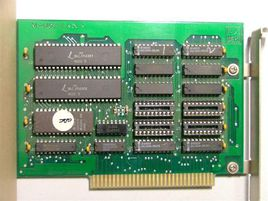
\includegraphics[scale=1.0]{\pythonroot/images/hanka.jpg}
  \caption{汉卡}
  \label{fig:hanka}
\end{figure}

\subsubsection{GBK}
GB2312 不能100\%满足中国汉字的需求,尤其是无法处理一些罕见的字和繁体字。
后来就在 GB2312 的基础上创建了一种叫 GBK 的编码。

GBK 编码标准,全称《汉字内码扩展规范》(GBK),英文名称 Chinese Internal Code Specification。
GB 即“国标”,K是“扩展”的汉语拼音第一个字母。
GBK 向下与 GB2312 编码兼容,向上支持 ISO 10646.1 国际标准,是前者向后者过度过程中的一个承上启下的标准。
GBK 共收录21886个汉字和图形符号,其中汉字(包括部首和构件)21003个,图形符号883个。
同时还包括 BIG5 中的全部汉字,并收录了藏文、蒙文、维吾尔文等主要的少数民族文字。
同样 GBK 也是兼容 ASCII 编码的,对于英文字符用1个字节来表示,汉字用两个字节来标识。

GBK 采用双字节表示,总体编码范围为 8140--FEFE 之间,首字节在 81--FE 之间,
尾字节在 40--FE 之间,剔除 XX7F 一条线。GBK 编码区分三部分:
\begin{enumerate}
  \item 汉字区,包括
      \begin{itemize}
        \item GBK/2:B0A1--F7FE, 收录 GB2312 汉字 6763 个,按原序排列;0x8140--A0FE,收录 CJK 汉字 6080 个;
        \item GBK/4:AA40--FEA0,收录 CJK 汉字和增补的汉字 8160 个。
      \end{itemize}
  \item 图形符号区,包括
      \begin{itemize}
        \item GBK/1:A1A1--A9FE,除 GB2312 的符号外,还增补了其它符号          
        \item GBK/5:A840--A9A0,扩除非汉字区。
      \end{itemize}
  \item 用户自定义区GBK 区域中的空白区,用户可以自己定义字符。
\end{enumerate}

\subsubsection{GB18030}
GB18030,全称:国家标准 GB18030-2005《信息技术中文编码字符集》,是中华人民共和国现时最新的内码字集,
是 GB18030-2000《信息技术信息交换用汉字编码字符集基本集的扩充》的修订版。

GB18030 与 GB2312-1980 和 GBK 兼容,共收录汉字70244个。
与 UTF 系列编码类似,GB18030 采用多字节编码,每个字可以由 1 个、2 个或 4 个字节组成。
编码空间庞大,最多可定义161万个字符。支持中国国内少数民族的文字,不需要动用造字区。
汉字收录范围包含繁体汉字以及日韩汉字 GB18030 编码是一二四字节变长编码。
\begin{enumerate}
  \item 单字节,其值从0到0x7F,与 ASCII 编码兼容。

  \item 双字节,第一个字节的值从 0x81 到 0xFE,第二个字节的值从 0x40 到 0xFE(不包括0x7F),与 GBK 标准兼容。

  \item 四字节,第一个字节的值从 0x81 到 0xFE,第二个字节的值从 0x30 到 0x39,
      第三个字节从 0x81 到 0xFE,第四个字节从 0x30 到 0x39。
\end{enumerate}

GB18030 可容纳的编码范围巨大, 基本上亚洲所有的少数民族的文字都包含在内了。

\subsubsection{Unicode}
虽然 GB2312、GBK、GB18030 很好的解决了汉字编码问题,但却不能走向国际舞台。
因为无论 GB2312 还是 GB18030,它们都是一种 “地区性DBCS”。
这导致了一个非常麻烦的问题,就是同一个文本文件可能因为编码集问题而在国外计算机中根本无法阅读。

全世界的文字有很多,不同的地区采用不同的编码方案,不利于信息的交流。
于是统一联盟国际组织决定着手解决这个问题,继而提出了Unicode编码
\footnote{可以在 \url{http://www.unicode.org/charts/} 查看 Unicode 与各地区的编码}。
Unicode的学名是“Universal Multiple-Octet Coded Character Set”,简称为UCS。
Unicode有两种格式:UCS-2 和 UCS-4。
UCS-2 就是用两个字节编码,一共16个比特位,这样最多可以表示65536个字符。
不过,要表示全世界所有的字符,显然65536个数字还远远不够,
因此 Unicode4.0 规范定义了一组附加的字符编码,UCS-4 就是用4个字节编码。
理论上完全可以涵盖一切语言所用的符号。世界上任何一个字符都可以用一个Unicode编码来表示,
一旦字符的Unicode编码确定下来后,就不会再改变了。

虽然 Unicode 帮我们解决了字符集统一的问题,但这并不是没有代价的。
Unicode 规定所有字符都必须用两字节来表示(即使是 ASCII 字符)。
由于“半角”英文符号只需要用到低8位,
所以其高8位永远是0,因此这种大气的方案在保存英文文本时会多浪费一倍的空间。

\subsubsection{UTF-8}
我们已经知道,英文字母只用一个字节表示就够了,如果 Unicode 统一规定,
每个符号用三个或四个字节表示,那么每个英文字母前都必然有两到三个字节是0,
这对于存储空间来说是极大的浪费,文本文件的大小会因此大出两三倍,这是难以接受的。
Unicode 在很长一段时间内无法推广,直到互联网的出现。
为解决unicode如何在网络上传输的问题,于是面向传输的众多 UTF(UCS Transfer Format)标准出现了。
常见的 UTF 格式有 UTF-8、UTF-16 和 UTF-32 等。
顾名思义,UTF-8就是每次8个位传输数据,而UTF-16就是每次16个位。
UTF-8 就是在互联网上使用最广的一种 Unicode 的实现方式,这是为传输而设计的编码,并使编码无国界,
这样就可以显示全世界上所有文化的字符了。

UTF-8最大的一个特点,就是它是一种变长的编码方式。
它可以使用 $1 \sim 4$ 个字节表示一个符号,根据不同的符号而变化字节长度。
当字符在 ASCII 码的范围时,就用一个字节表示,保留了 ASCII 字符一个字节的编码做为它的一部分
(注意的是 Unicode 一个中文字符占2个字节,而 UTF-8 一个中文字符占3个字节)。
对于多字节($n$ 个字节)的字符,第一个字节的前 $n$ 位都设为1,第 $n + 1$ 位设为0,
后面字节的前两位都设为10。剩下的二进制位全部用该字符的 Unicode 码填充。
具体的转换规则如表\ref{table:utf8-coding}所示
\footnote{可以在 \url{http://www.qqxiuzi.cn/bianma/Unicode-UTF.php} 查看 Unicode 与 UTF-8 编码转换}。

\begin{table}[!htb]
  \centering
  \begin{tabular}{|Sc|l|}
    \hline
    \tableheadcolor \textbf{Unicode符号范围(十六进制)} & \textbf{UTF-8编码方式(二进制)} \\ \hline
    0000 0000 -- 0000 007F & 0xxxxxxx \\ \hline
    0000 0080 -- 0000 07FF & 110xxxxx 10xxxxxx \\ \hline
    0000 0800 -- 0000 FFFF & 1110xxxx 10xxxxxx 10xxxxxx \\ \hline
    0001 0000 -- 0010 FFFF & 11110xxx 10xxxxxx 10xxxxxx 10xxxxxx \\ \hline
  \end{tabular}
  \caption{UTF-8编码方式}
  \label{table:utf8-coding}
\end{table}

以汉字“解”为例,“解”对应的 Unicode 是89E3,对应的区间是0000 0800 -- 0000 FFFF,
因此它用 UTF-8 表示时需要用3个字节来存储,89E3 用二进制表示是:1000 1001 1110 0011,
填充到 1110xxxx 10xxxxxx 10xxxxxx 得到 1110\textbf{1000} 10\textbf{100111} 10\textbf{100011},
转换成16进制:E8A7A3。因此“解”的 Unicode “89E3” 对应的 UTF-8 编码是“E8A7A3”。

\begin{table}[!htb]
  \centering
    \begin{tabular}{|>{\columncolor{SeaGreen3!30!}}Sr|l|}
    \hline
    \textbf{中文} & 解 \\ \hline
    \textbf{Unicode} & \qquad 1000 \quad 100111 \quad 100011 \\ \hline
    \textbf{编码规则} & 1110xxxx 10xxxxxx 10xxxxxx \\ \hline
    \textbf{UTF-8} &    11101000 10100111 10100011 \\ \hline
    \textbf{16进制UTF-8} & \ \ \,E \quad\,8 \quad\ \,A \quad 7 \quad\ \,A \quad\,3 \\ \hline
  \end{tabular}
  \caption{中文“解”的 UTF-8 编码}
  \label{table:jie-utf8-coding}
\end{table}

\paragraph*{相关资料}
文本编码是一个极其常见的问题,网络上也有大量相关的材料和讨论。推荐阅读下列材料:
\begin{enumerate}
  \item \href{https://www.zhihu.com/question/19677619}{知乎:GB2312、GBK、GB18030 这几种字符集的主要区别是什么?}
  \item \href{http://web.jobbole.com/89552/}{前端历史课:那些来自洪荒时代的编码知识}
\end{enumerate}

\subsection{Python编码}

\subsubsection{Python2}
Python 是 Guido van Rossum 在1992年创造的,那时的 Unicode 还没有发布,
而 Guido 绝对没想到 Python 这门语言在今天会如此受大家欢迎。
因此,在 Python2 中默认编码为 ASCII 码,有两种字符序列类型:str 和 unicode 类型,
它们都是 basestring 的子类。Python2 中还有一个 bytes 类型,与 str 等价。
可以通过代码 \ref{code:Python2-defaultencoding} 获取默认编码。

\begin{jcode}{python}{获取 Python2 默认编码}{code:Python2-defaultencoding}
Python 2.7.15 (default, May  1 2018, 16:44:08)
[GCC 4.2.1 Compatible Apple LLVM 9.1.0 (clang-902.0.39.1)] on darwin
Type "help", "copyright", "credits" or "license" for more information.
>>> import sys
>>> sys.getdefaultencoding()
'ascii'
>>> s = "解惑者"
>>> type(s)
<type 'str'>
>>> s
'\xe8\xa7\xa3\xe6\x83\x91\xe8\x80\x85'
>>>
\end{jcode}

在 Python2 源代码文件中如果不显示地指定编码的话,将出现语法错误。

\begin{jcode}{python}{Python2 不指定编码}{code:Python2-coding-exception}
# test_encoding_exception.py
print("解惑者")
\end{jcode}

运行 \ref{code:Python2-coding-exception} 中的代码,将出现如下错误:
\begin{quote}
File ``test.py", line 2

SyntaxError: Non-ASCII character `$\backslash$ xe8' in file test.py on line 2, but no encoding declared; see http://python.org/dev/peps/pep-0263/ for details
\end{quote}

为了在源代码中支持非 ASCII 字符,必须在源文件的第一行或者第二行显示地指定编码格式
(参考代码 \ref{code:Python2-set-file-encoding-1} 和 代码 \ref{code:Python2-set-file-encoding-2})。

\begin{jcode}{python}{Python2 指定编码格式}{code:Python2-set-file-encoding-1}
# coding=utf-8
\end{jcode}

\begin{jcode}{python}{Python2 指定编码格式}{code:Python2-set-file-encoding-2}
# -*- coding: utf-8 -*-
\end{jcode}

对于同一个汉字“解”,用 str 表示时,它对应的就是 utf-8 编码为 `E8A7A3',
而用 unicode 表示时,它对应的符号就是 u`89E3',与 u`解' 是等同的。
那么在 Python2 中 str 和 unicode 之间是如何转换的呢?
这两种类型的字符串类型之间的转换就是靠这两个方法 decode 和 encode,具体见图\ref{fig:Python2-str-2-unicode}。

\begin{figure}[ht]
  \centering
  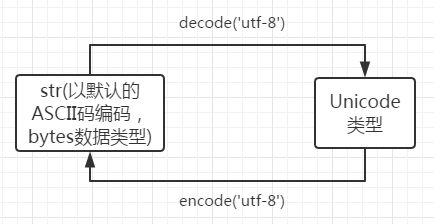
\includegraphics[scale=0.4]{\pythonroot/images/py2_str2unicode.jpg}
  \caption{Python2 str 与 unicode 的转换}
  \label{fig:Python2-str-2-unicode}
\end{figure}

代码 \ref{code:Python2-str-2-unicode} 中解释了如何在 str 和 unicode 类型之间做转换。

\begin{jcode}{python}{Python2 str 和 unicode 类型之间的转换}{code:Python2-str-2-unicode}
#从str类型转换到unicode
s.decode(encoding)   =====>  <type 'str'> to <type 'unicode'>
#从unicode转换到str
u.encode(encoding)   =====>  <type 'unicode'> to <type 'str'>

>>> su = u"解" 
>>> ss = su.encode('utf-8')
>>> type(ss)
<type 'str'>
>>> ss
'\xe8\xa7\xa3'

>>> sc = ss.decode('utf-8')
>>> type(sc)
<type 'unicode'>
>>> sc
u'\u89e3'
\end{jcode}

str(s) 和 unicode(s) 是两个工厂方法,分别返回 str 字符串对象和 unicode 字符串对象。

\begin{jcode}{python}{Python2 str(s)方法}{code:Python2-str-s-ascii}
>>> s3 = u"解惑者"
>>> s3
u'\u89e3\u60d1\u8005'
>>> str(s3)
Traceback (most recent call last):
  File "<stdin>", line 1, in <module>
UnicodeEncodeError: 'ascii' codec can't encode characters in position 0-2:
ordinal not in range(128)
\end{jcode}

上面 s3 是 unicode 类型的字符串,str(s3) 相当于是执行s3.encode(`ascii')。
因为“解惑者”三个汉字不能用 ascii 码来表示,所以就报错了。
指定正确的编码:s3.encode(`gbk') 或者 s3.encode(`utf-8') 就不会出现这个问题了。
类似的unicode有同样的错误:
\begin{jcode}{python}{Python2 unicode(s)方法}{code:Python2-unicode-s-ascii}
>>> s4 = "解惑者"
>>> unicode(s4)
Traceback (most recent call last):
  File "<stdin>", line 1, in <module>
UnicodeDecodeError: 'ascii' codec can't decode byte 0xe8 in position 0:
ordinal not in range(128)
>>>
\end{jcode}

unicode(s4) 等效于 s4.decode(`ascii'),
因此要正确的转换就要正确指定其编码 s4.decode(`gbk') 或者 s4.decode(`utf-8')。

从上面使用 str(s) 和 unicode(s) 的示例中,我们自然会想到另外一个问题:如果我们对
unicode 变量使用 decode 方法,对 str 变量使用 encode 方法会怎么样?

\begin{jcode}{python}{Python2 encode decode}{code:Python2-encode-decode}
>>> s = u"解惑者"
>>> s
u'\u89e3\u60d1\u8005'
>>> s.decode('utf-8')
Traceback (most recent call last):
  File "<stdin>", line 1, in <module>
  File "PythonPath/Versions/2.7/lib/python2.7/encodings/utf_8.py", line 16, in decode
    return codecs.utf_8_decode(input, errors, True)
UnicodeEncodeError: 'ascii' codec can't encode characters in position 0-2:
ordinal not in range(128)
>>>
>>> s = "解惑者"
>>> s
'\xe8\xa7\xa3\xe6\x83\x91\xe8\x80\x85'
>>> s.encode('utf-8')
Traceback (most recent call last):
  File "<stdin>", line 1, in <module>
UnicodeDecodeError: 'ascii' codec can't decode byte 0xe8 in position 0:
ordinal not in range(128)
>>>
\end{jcode}

对于代码 \ref{code:Python2-encode-decode} 的前半部分,由于 s 是 unicode 变量,
因此 s.decode(`utf-8') 相当于 s.encode().decode(`utf-8'),但 s 并不是一个有效的 ascii 编码字符。
同样,对于代码 \ref{code:Python2-encode-decode} 的后半部分,由于 s 是一个 str 变量,
因此 s.encode(`utf-8') 相当于 s.decode().encode(`utf-8'),但显然 s 并不能用 ascii 解码。

从上面的示例也可以看出,Python2 并没有严格区分字符流和字节流,
因此 encode 和 decode 方法的使用比较混乱,导致使用时可能出现各种问题。
Python3 则严格区分了字符流和字节流,不会有这类问题。

如果不想使用 GBK、utf-8 这些编码,而直接使用 unicode 编码,那么应该怎么做呢?
在 Python 中 unicode 字符集表示为 `unicode-escape' 编码集。
与 GBK、utf-8 编码类似,对于 unicode 编码的字符串,可以使用 decode 进行解码,
见代码\ref{code:Python2-unicode-str-decode}。

\begin{jcode}{python}{Python2 unicode解码}{code:Python2-unicode-str-decode}
>>> s = 'id\u003d215903184\u0026index\u003d0\u0026st\u003d52\u0026sid\u003d95000'
>>> print(type(s))
<type 'str'>
>>> s = s.decode('unicode-escape')
>>> s
u'id=215903184&index=0&st=52&sid=95000'
>>> print(type(s))
<type 'unicode'>
>>>
\end{jcode}

拓展:还有一种 string-escape 编码集,可以对字节流用 string-escape 进行编码。

\subsubsection{Python3}
Python2 的字符串编码经常会让人误解,因此 Python3 对字符串编码进行了重新设计。
在 Python3 当中,文本字符串类型(使用 unicode 数据存储)被命名为 str,字节字符串类型被命名为 bytes,
二者的转换关系如图 \ref{fig:Python3-str-2-bytes} 所示。

\begin{figure}[ht]
  \centering
  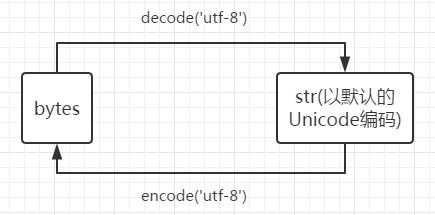
\includegraphics[scale=0.4]{\pythonroot/images/py3_bytes2str.jpg}
  \caption{Python3 str 与 bytes 的转换}
  \label{fig:Python3-str-2-bytes}
\end{figure}

一般情况下,实例化一个字符串会得到一个 str 对象。需要注意的是,这里的 str 对象,
与 Python2 的 unicode 对象类似,均使用 unicode 编码。

\begin{jcode}{python}{Python3 实例化字符串}{code:Python3-str-init}
Python 3.6.5 (v3.6.5:f59c0932b4, Mar 28 2018, 03:03:55)
[GCC 4.2.1 (Apple Inc. build 5666) (dot 3)] on darwin
Type "help", "copyright", "credits" or "license" for more information.
>>> s = "解惑者"
>>> type(s)
<class 'str'>
>>> s
'解惑者'
>>>
\end{jcode}

所以 Python3 也可以认为是默认使用 unicode 编码。
如果你想得到bytes,那就在文本之前加上前缀 b , 或者 encode 一下。

\begin{jcode}{python}{Python3 encode方法示例}{code:Python3-encode}
>>> s.encode('GBK')
b'\xbd\xe2\xbb\xf3\xd5\xdf'
>>> s.encode('utf-8')
b'\xe8\xa7\xa3\xe6\x83\x91\xe8\x80\x85'
>>> a = b'hello'
>>> a.__repr__()
"b'hello'"
>>>
\end{jcode}

所以,很显然,str 对象有一个encode方法,bytes 对象有一个decode方法。
需要注意的是,对于 Python2 来说,无论是 str 还是 unicode,均有 encode 和 decode 方法,
这样就把字符串与字节流混淆了,但str(与Python3的bytes类似)的decode 和
unicode(与Python3的unicode类似)的 encode 方法本身并没有什么太大的作用。
Python3 里考虑到了这个特点,因此 str 只有 encode 方法,bytes 只有 decode 方法。

\section{常用内置库}

\subsection{logging}


\section{常用第三方库}

\subsection{YAML}
github主页:\href{https://github.com/yaml}{The YAML Project}

假设你有一个YAML配置文件,其内容如\ref{code:yaml-simple-config}所示。

\begin{jcode}{yaml}{YAML代码示例}{code:yaml-simple-config}
# tree format
treeroot:
    branch1:
        name: Node 1
        branch1-1:
            name: Node 1-1
    branch2:
        name: Node 2
        branch2-1:
            name: Node 2-1
\end{jcode}

可以通过\ref{code:yaml-simple-usage}的代码获取配置文件的内容。

\begin{jcode}{python}{YAML代码示例}{code:yaml-simple-usage}
import yaml
with open('config.yaml') as f:
    # use safe_load instead load
    conf = yaml.safe_load(f)
\end{jcode}

如果想要将现有的项保存成 YAML 文件,则可以采用类似于 \ref{code:yaml-simple-saving} 的代码。
\begin{jcode}{python}{保存配置到YAML文件中}{code:yaml-simple-saving}
with open('config.yaml', "w") as f:
    yaml.dump(conf, f)
\end{jcode}

\subsection{requests}

\subsection{numpy}
NumPy系统是Python的一种开源的数值计算扩展。这种工具可用来存储和处理大型矩阵,比Python自身的嵌套列表结构要高效的多。

\begin{minted}[mathescape,
               numbersep=5pt,
               frame=lines,
               framesep=2mm]{python}
>>> import numpy as np
>>> np.array(3).shape
()
>>> np.array([1]).shape
(1,)
>>> np.array([1, 2, 3]).shape
(3,)
>>> np.array([[1, 2, 3], [4, 5, 6]]).shape
(2, 3)
>>> np.array([[[1, 2, 3], [4, 5, 6]], [[7, 8, 9], [10, 11, 12]]]).shape
(2, 2, 3)
\end{minted}

\begin{minted}[mathescape,
               numbersep=5pt,
               frame=lines,
               framesep=2mm]{python}
>>> import numpy as np
>>> a = np.zeros((3, 3))
>>> a
array([[ 0.,  0.,  0.],
       [ 0.,  0.,  0.],
       [ 0.,  0.,  0.]])
>>> import numpy as np
>>> a = np.ones((3, 3))
>>> a
array([[ 1.,  1.,  1.],
       [ 1.,  1.,  1.],
       [ 1.,  1.,  1.]])
>>> import numpy as np
>>> a = np.full((3, 3), 5)
>>> a
array([[5, 5, 5],
       [5, 5, 5],
       [5, 5, 5]])
\end{minted}


\begin{minted}[mathescape, numbersep=5pt, frame=lines, framesep=2mm]{python}
>>> import numpy as np
>>> a = np.array([1, 2, 3, 4, 5, 6, 7, 8, 9])
>>> a[:3]
array([1, 2, 3])
>>> a[5:]
array([6, 7, 8, 9])
>>> a[5:8]
array([6, 7, 8])
>>> a[5]
6
>>> a[-1]
9
>>> a[-2]
8
\end{minted}


\begin{minted}[mathescape, numbersep=5pt, frame=lines, framesep=2mm]{python}
>>> import numpy as np
>>> a = np.array([[1, 2, 3], [4, 5, 6], [7, 8, 9]])
>>> a[0:2, 0:2]
array([[1, 2],
       [4, 5]])
>>> a[1, 1]
5
\end{minted}


\begin{minted}[mathescape, numbersep=5pt, frame=lines, framesep=2mm]{python}
>>> import numpy as np
>>> a = np.array([[1, 2], [3, 4], [5, 6]])
>>> index = (a > 2)
>>> print(index)
[[False False]
 [ True  True]
 [ True  True]]
>>> print(a[index])
[3 4 5 6]
>>> print(a[a > 2])
[3 4 5 6]
\end{minted}


\begin{minted}[mathescape, numbersep=5pt, frame=lines, framesep=2mm]{python}
>>> import numpy as np
>>> a = np.array([1, 2, 3, 4])
>>> b = np.array([2, 3, 4, 5])
>>> c = a * b
>>> c
array([ 2,  6, 12, 20])
\end{minted}

\begin{minted}[mathescape, numbersep=5pt, frame=lines, framesep=2mm]{python}
>>> import numpy as np
>>> a = np.array([1, 2, 3, 4])
>>> b = np.array([2, 3, 4, 5])
>>> c = np.multiply(a, b)
>>> c
array([ 2,  6, 12, 20])
\end{minted}

\begin{minted}[mathescape, numbersep=5pt, frame=lines, framesep=2mm]{python}
>>> import numpy as np
>>> a = np.array([[1, 2, 3], [4, 5, 6]])
>>> b = np.array([[6, 5], [4, 3], [2, 1]])
>>> c = a.dot(b)
>>> c
array([[20, 14],
       [56, 41]])
\end{minted}

\begin{minted}[mathescape, numbersep=5pt, frame=lines, framesep=2mm]{python}
>>> import numpy as np
>>> a = np.array([[1, 2], [3, 4]])
>>> np.sum(a)
10
>>> np.sum(a, axis=1)
array([3, 7])
>>> np.sum(a, axis=0)
array([4, 6])
\end{minted}

\begin{minted}[mathescape, numbersep=5pt, frame=lines, framesep=2mm]{python}
>>> import numpy as np
>>> a = np.array([[1, 2], [3, 4]])
>>> np.max(a)
4
>>> np.max(a, axis=0)
array([3, 4])
>>> np.max(a, axis=1)
array([2, 4])
\end{minted}

\begin{minted}[mathescape, numbersep=5pt, frame=lines, framesep=2mm]{python}
>>> import numpy as np
>>> a = np.array([[1, 2], [3, 4]])
>>> np.min(a)
1
>>> np.min(a, axis=0)
array([1, 2])
>>> np.min(a, axis=1)
array([1, 3])
\end{minted}

\begin{minted}[mathescape, numbersep=5pt, frame=lines, framesep=2mm]{python}
>>> import numpy as np
>>> a = np.array([1, 2, 3, 4, 5, 6])
>>> a.reshape((2, 3))
array([[1, 2, 3],
       [4, 5, 6]])
>>> a.reshape((3, 2))
array([[1, 2],
       [3, 4],
       [5, 6]])
\end{minted}

\begin{minted}[mathescape, numbersep=5pt, frame=lines, framesep=2mm]{python}
>>> import numpy as np
>>> a = np.array([1, 2, 3, 4, 5, 6])
>>> b = a.reshape((3, 2))
>>> b
array([[1, 2],
       [3, 4],
       [5, 6]])
>>> b.flatten()
array([1, 2, 3, 4, 5, 6])
\end{minted}

\begin{minted}[mathescape, numbersep=5pt, frame=lines, framesep=2mm]{python}
>>> import numpy as np
>>> a = np.array([[1, 2], [3, 2]])
>>> a
array([[1, 2],
       [3, 2]])
>>> a.T
array([[1, 3],
       [2, 2]])
\end{minted}


\begin{minted}[mathescape, numbersep=5pt, frame=lines, framesep=2mm]{python}
from sklearn.linear_model import LogisticRegression
lr_model = LogisticRegression()

>>> from sklearn import datasets
>>> iris = datasets.load_iris()
>>> digits = datasets.load_digits()


from sklearn.metrics import SCORERS
for i in SCORERS.keys():
    print(i)

from __future__ import print_function
from sklearn import datasets
from sklearn.cross_validation import train_test_split
from sklearn.neighbors import KNeighborsClassifier

>>> from __future__ import print_function
>>> from sklearn import datasets
>>> from sklearn.cross_validation import train_test_split
>>> from sklearn.neighbors import KNeighborsClassifier
>>> 
>>> 
>>> iris = datasets.load_iris()
>>> iris_X = iris.data
>>> iris_y = iris.target
>>> 
>>> X_train, X_test, y_train, y_test = train_test_split(iris_X, iris_y, test_size=0.3)
>>> 
>>> knn = KNeighborsClassifier()
>>> knn.fit(X_train, y_train)
KNeighborsClassifier(algorithm='auto', leaf_size=30, metric='minkowski',
           metric_params=None, n_jobs=1, n_neighbors=5, p=2,
           weights='uniform')
>>> print(knn.predict(X_test))
[0 0 0 1 2 0 2 1 2 1 1 2 0 2 1 2 1 0 1 0 2 1 0 0 2 1 2 2 1 1 0 1 1 1 0 1 2
 2 1 2 0 1 0 1 0]
>>> print(y_test)
[0 0 0 1 1 0 2 1 2 2 1 2 0 2 1 2 1 0 1 0 2 1 0 0 2 1 2 2 1 1 0 1 1 1 0 1 2
 2 1 2 0 1 0 1 0]
\end{minted}

\ifx\engineeringnotes\undefined
    \bibliography{\notesroot/reference/reference.bib}
\end{document}

\fi
